% MARINA VON STEINKIRCH, SPRING/2013
% http://mysbfiles.stonybrook.edu/~mvonsteinkir/
\documentclass[11pt]{article}

\usepackage{epsfig}
\usepackage{color}
\usepackage{amsmath}    % Package  for subequations
\usepackage{graphicx}   % Package for figures
\usepackage{verbatim}   % Package  for program listings
\usepackage{hyperref}   % Package  for hypertext links, external documents and URLs
\usepackage{amssymb} % For mathematical constructions
\usepackage{latexsym} % Package to generate mathematical symbols
\usepackage{makeidx} % Package to generate an index in the end
\usepackage{float}

\newcommand{\ie}{{\it i.e., }}
\newcommand{\eg}{{\it e.g., }}


\title{CSE 590: Computational Photography\\  Homework \#3: Face Morphism }
\author{ \texttt{ Marina von Steinkirch, steinkirch@gmail.com}\\
	   \texttt{State University of New York at Stony Brook}}
\date{\today}




\begin{document}
\maketitle
\numberwithin{equation}{section}  




\section{Introduction}


A {\it morph} is a simultaneous warp of the image shape and a cross-dissolve of the image colors. The warp is controlled by defining a correspondence between two pictures (\eg the map between eyes, mouths, etc.). 


\quad

In this work we describe the technique to morph two face images using {\it Delaunay Triangulation} and we apply the method to compute a {\it mean face} for many face images. In addition, we further illustrate this technique on fun examples such as caricatures and the transformation of a face to a zombie.

\newpage




\section{Labeling Points in a Face Image}

To establish the connection between face images we label 43 corresponding points (\ie eye to eyes, month to month, etc) using a frame as a reference (\eg see Fig. \ref{pointslabel}). In MATLAB we can perform this task by two ways: using the function \texttt{cpselect()} or using the function \texttt{ginput()}. Both options return same results and precision (and are include in the  source code).


\quad

\begin{figure} [ht]
\begin{center}
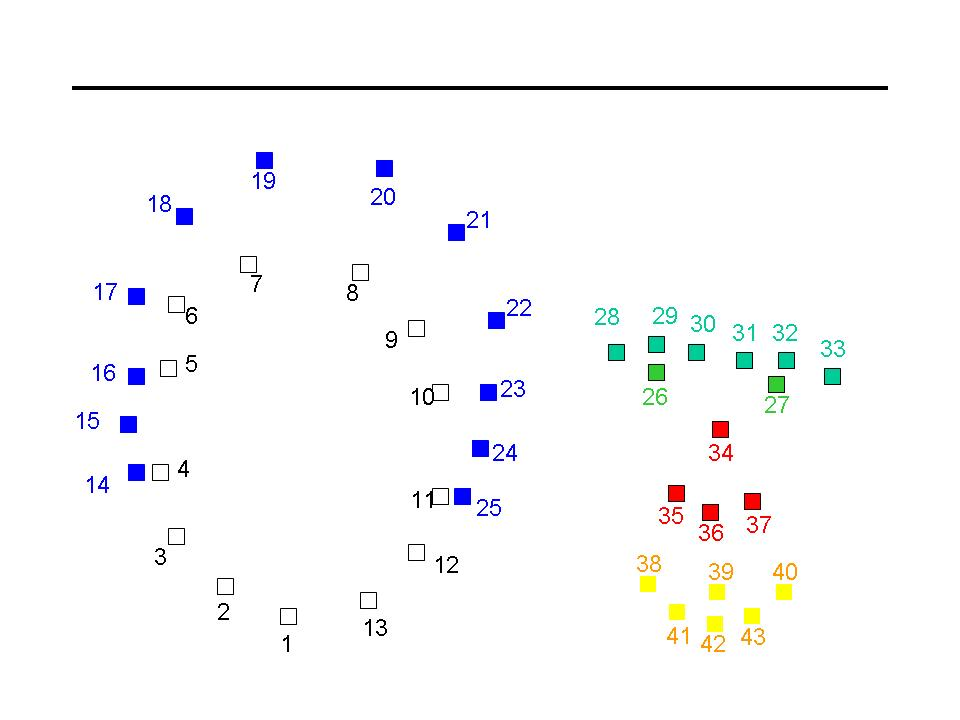
\includegraphics[scale=0.3]{figs/pointlabels.jpg}  
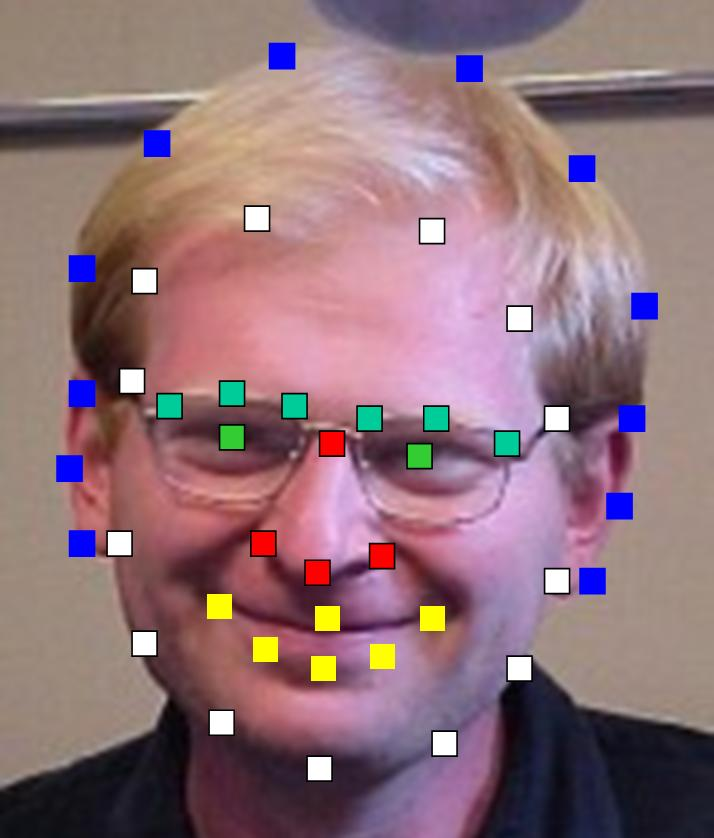
\includegraphics[scale=0.3]{figs/efros.jpg}  
\includegraphics[scale=0.3]{figs/melabel.png}  
\caption{Example of how to label/map points in the face images: the mapping and an example from  \cite{tamara} and how it worked for the image face.}
\label{pointslabel}
\end{center}
\end{figure}


\newpage



\section{Delaunay Triangulation}

With the labeled points from the previous step, we were able to apply the techniques of face morphism to two face images. For this purpose, we chose the triangulation method given by {\it Delaunay triangulation}, which  does not produce overly acute triangles. 

\quad

The triangulation was computed to the {\it mean of the two point sets} (the midway shape) since they must be the same throughout the morph. Doing so in this fashion, we reduced the potential triangle deformations. Triangulation results are shown in the Fig. \ref{triang}.

\quad

\begin{figure} [ht]
\begin{center}
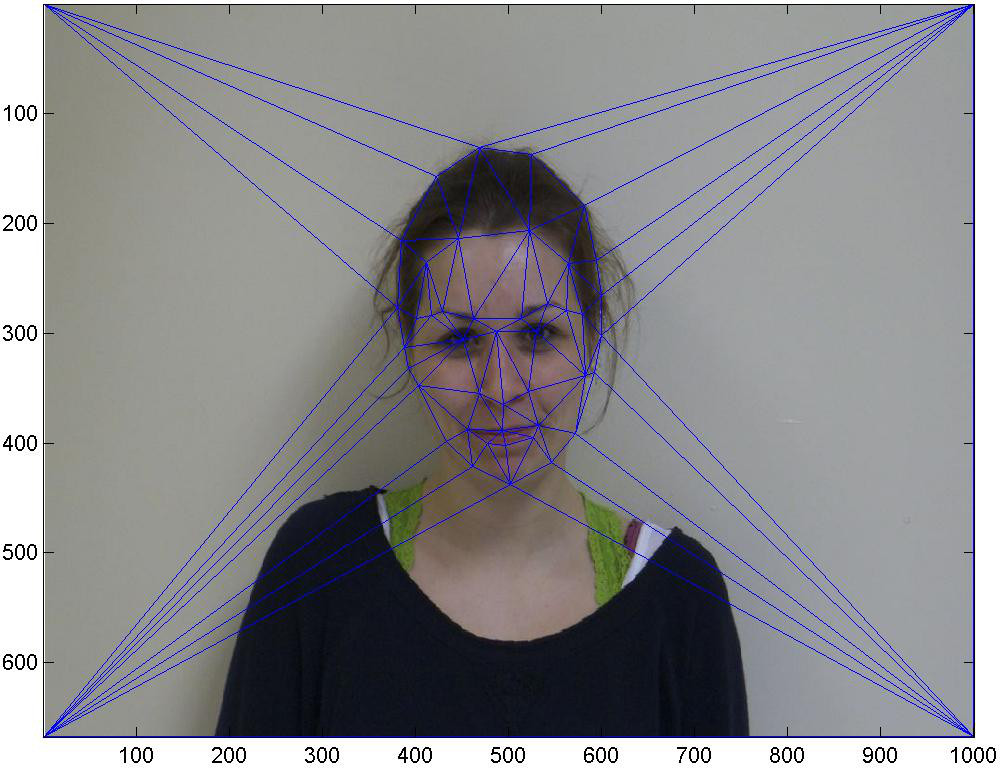
\includegraphics[scale=0.1]{figs/triang/1.jpg}  
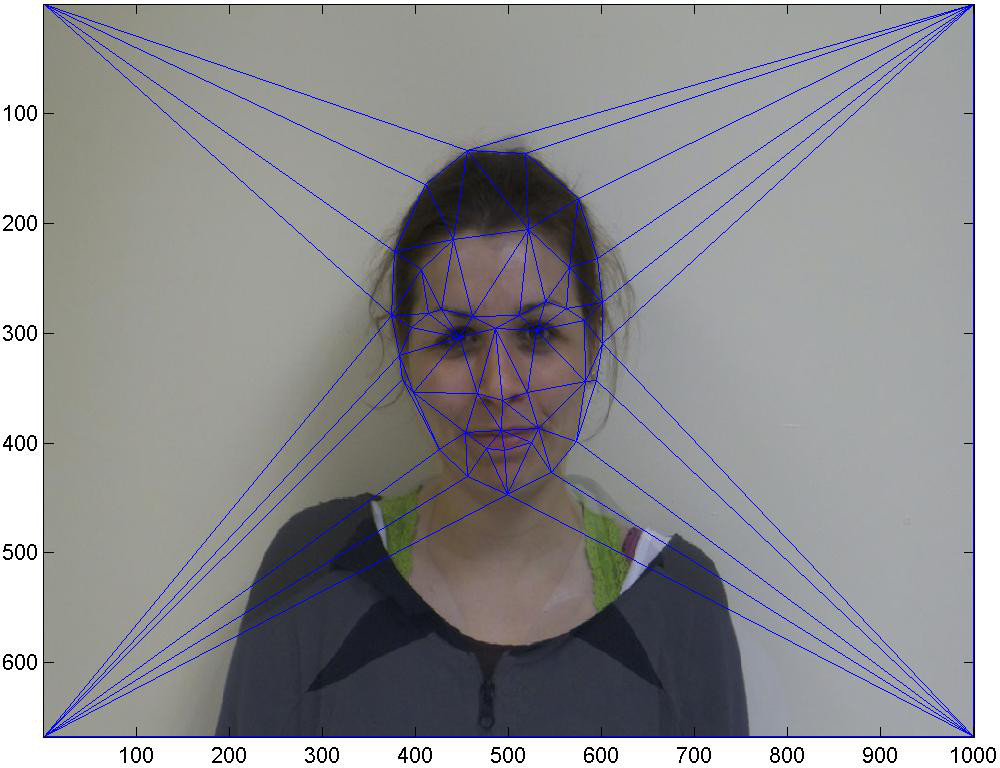
\includegraphics[scale=0.1]{figs/triang/3.jpg}  
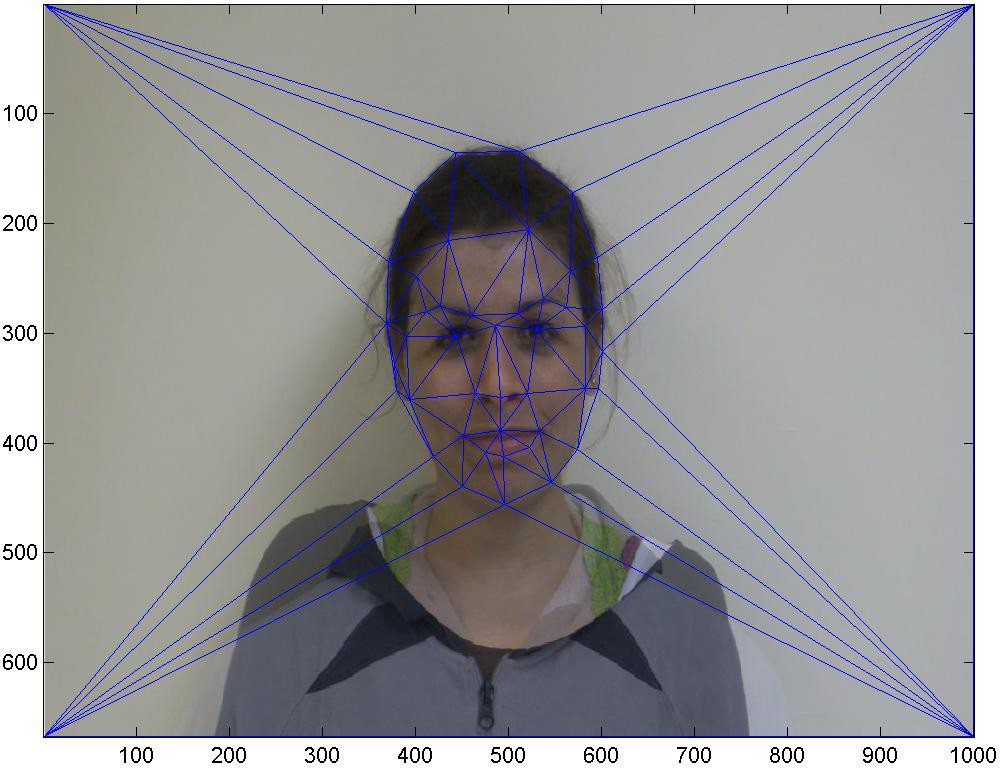
\includegraphics[scale=0.1]{figs/triang/5.jpg}  
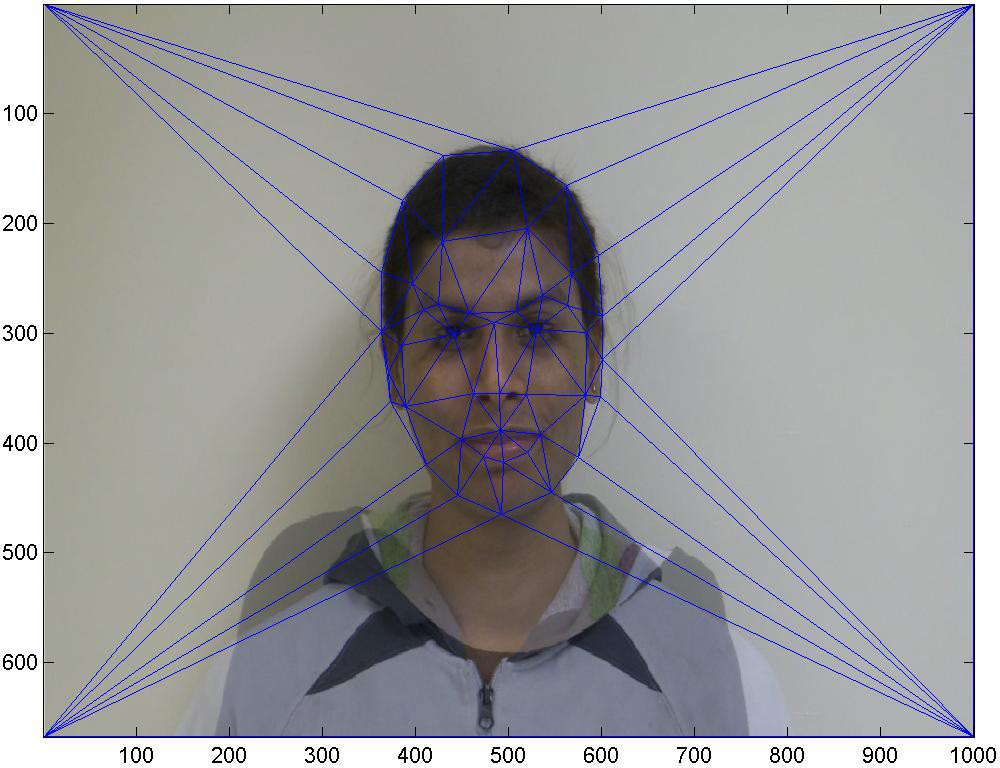
\includegraphics[scale=0.1]{figs/triang/6.jpg}  
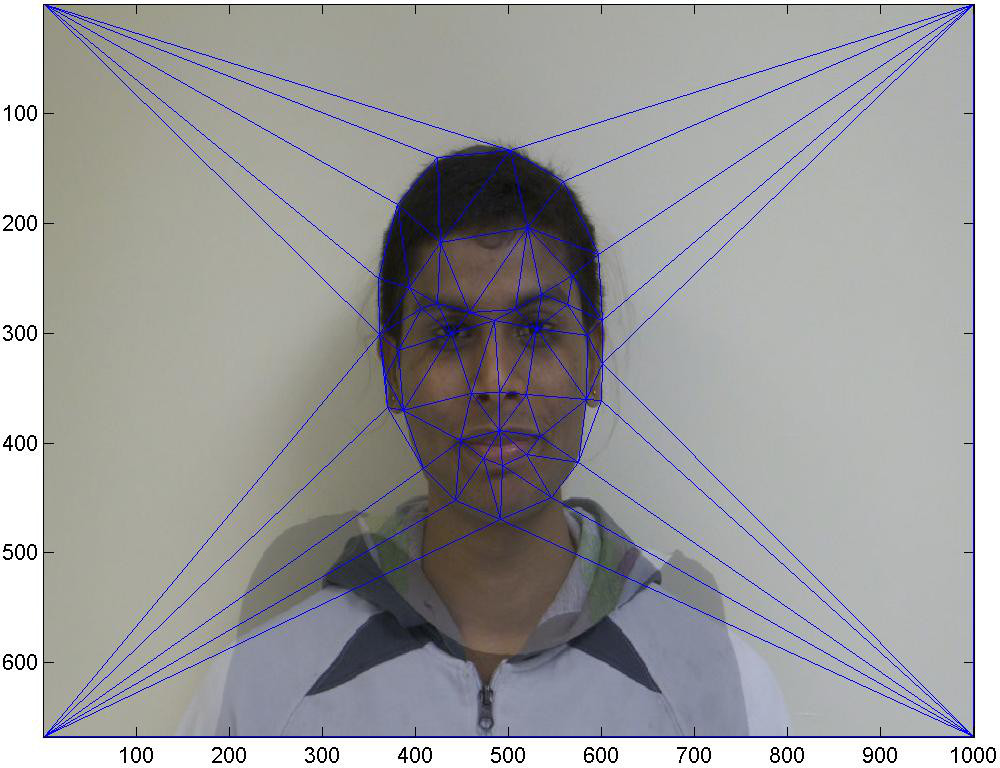
\includegraphics[scale=0.1]{figs/triang/7.jpg}  
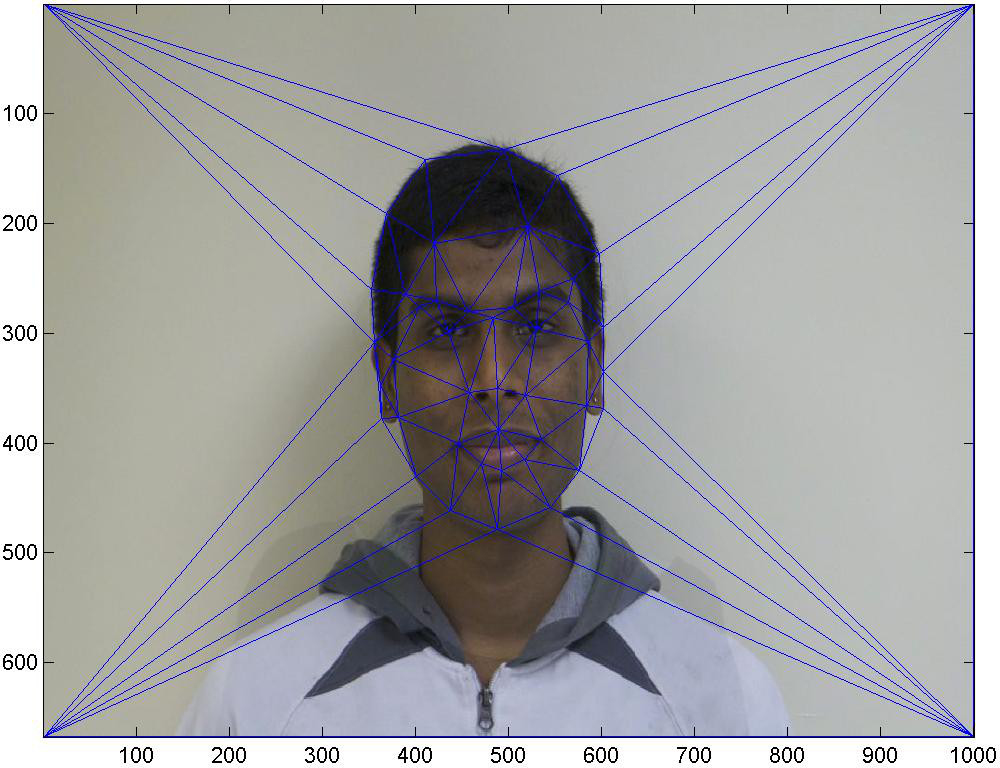
\includegraphics[scale=0.1]{figs/triang/9.jpg}  
\caption{Delaunay triangulation for many of the intermediate steps during the face morphism process.}
\label{triang}
\end{center}
\end{figure}



\newpage


\section{Defining Correspondences and Warping Faces}

For each {\it morphed frame} we:

\begin{enumerate}
\item Interpolate geometry by weighted average of point locations;
\item Warp each image to the interpolated geometry by finding affine warps between triangles and doing affine projections on points;
\item Linearly blend warped images as a weighted average.
\end{enumerate}

\quad

As a result, we generate 60 intermediate frames that smoothly map the original face image to the final face image. The process is shown in the Fig. \ref{frames} and a video with the result can be seen at \cite{video-face}.




\begin{figure}[H]
\begin{center}

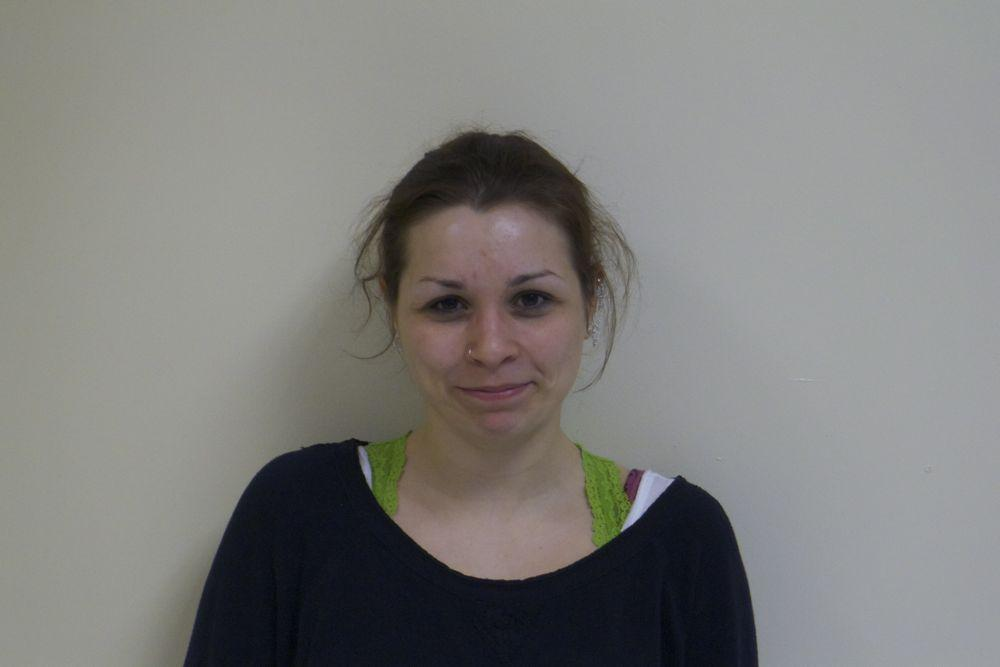
\includegraphics[scale=0.06]{figs/frames/morph_steinkirch_tangatur_01.jpg}  
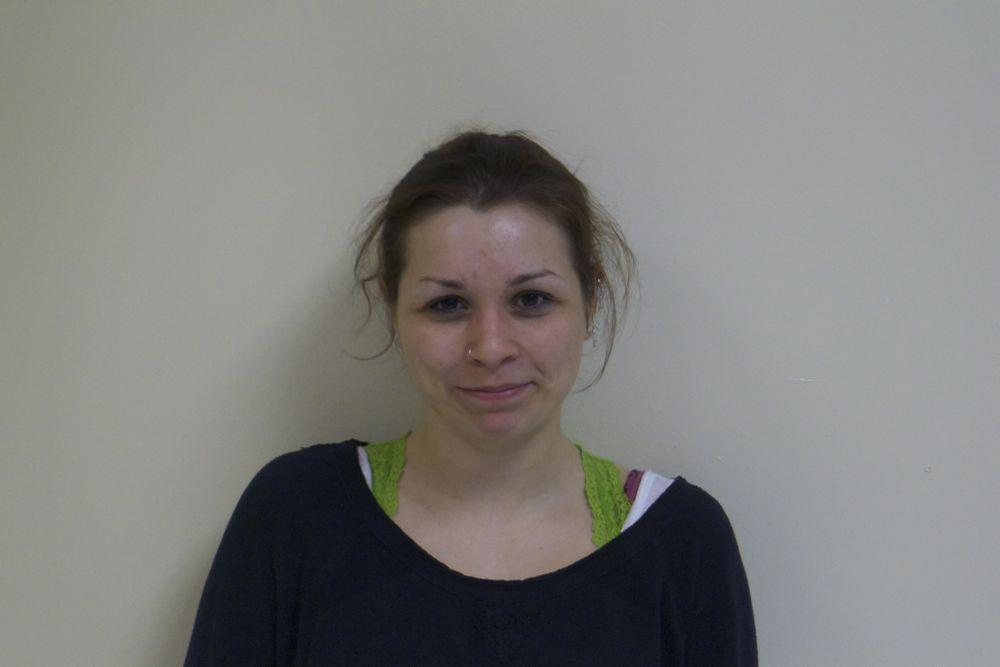
\includegraphics[scale=0.06]{figs/frames/morph_steinkirch_tangatur_02.jpg} 
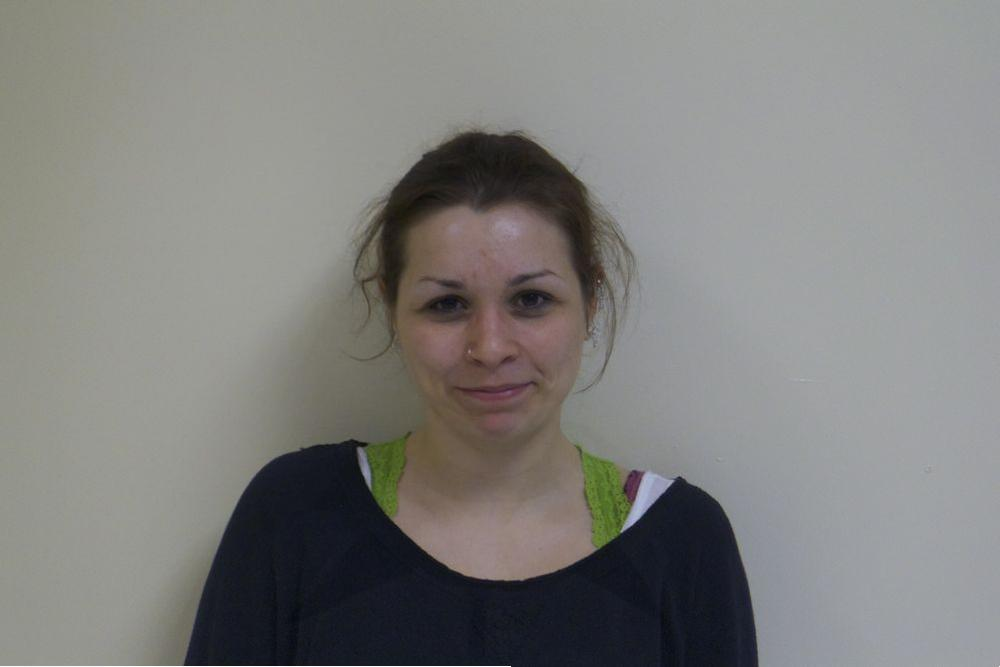
\includegraphics[scale=0.06]{figs/frames/morph_steinkirch_tangatur_03.jpg} 
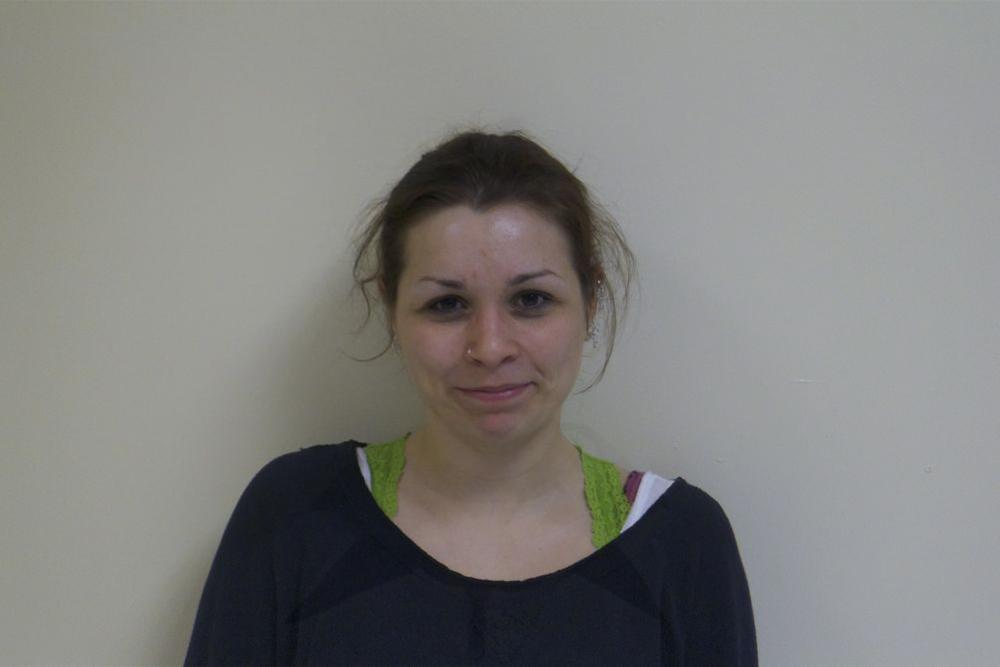
\includegraphics[scale=0.06]{figs/frames/morph_steinkirch_tangatur_04.jpg} 
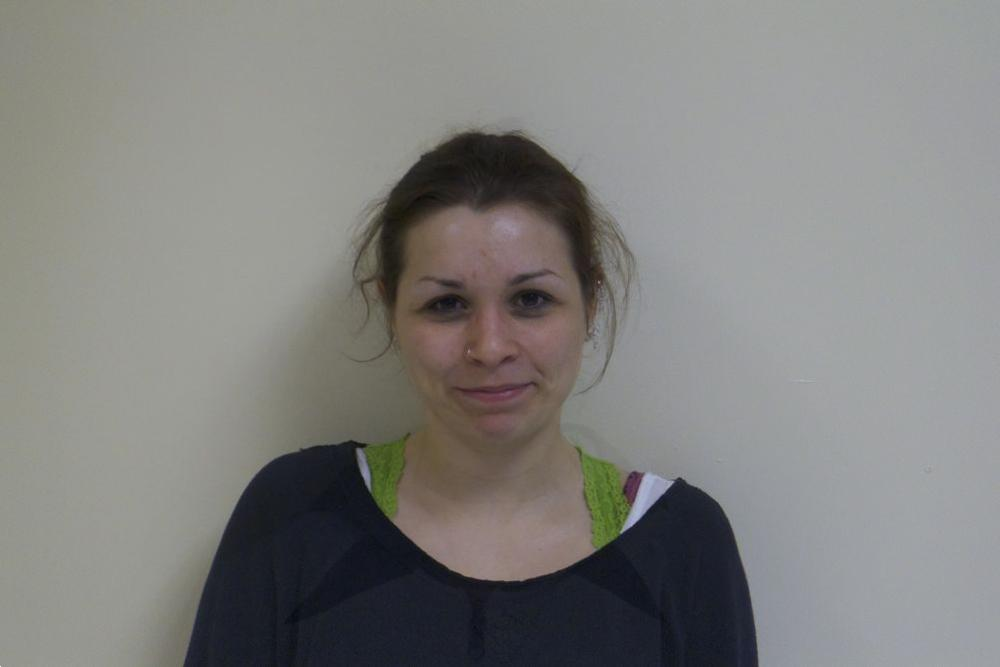
\includegraphics[scale=0.06]{figs/frames/morph_steinkirch_tangatur_05.jpg} 
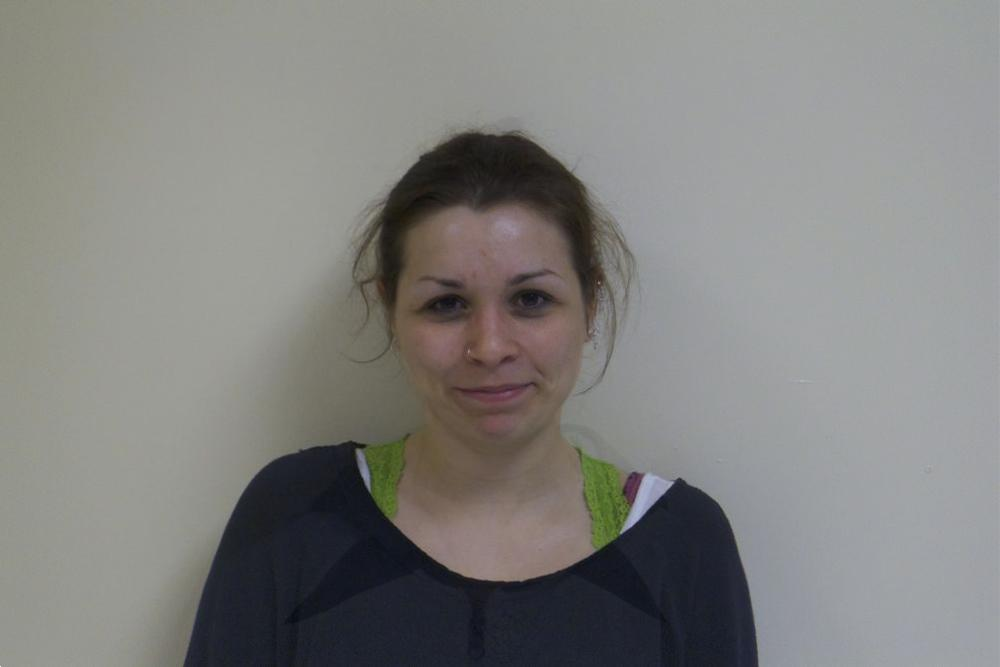
\includegraphics[scale=0.06]{figs/frames/morph_steinkirch_tangatur_06.jpg} 
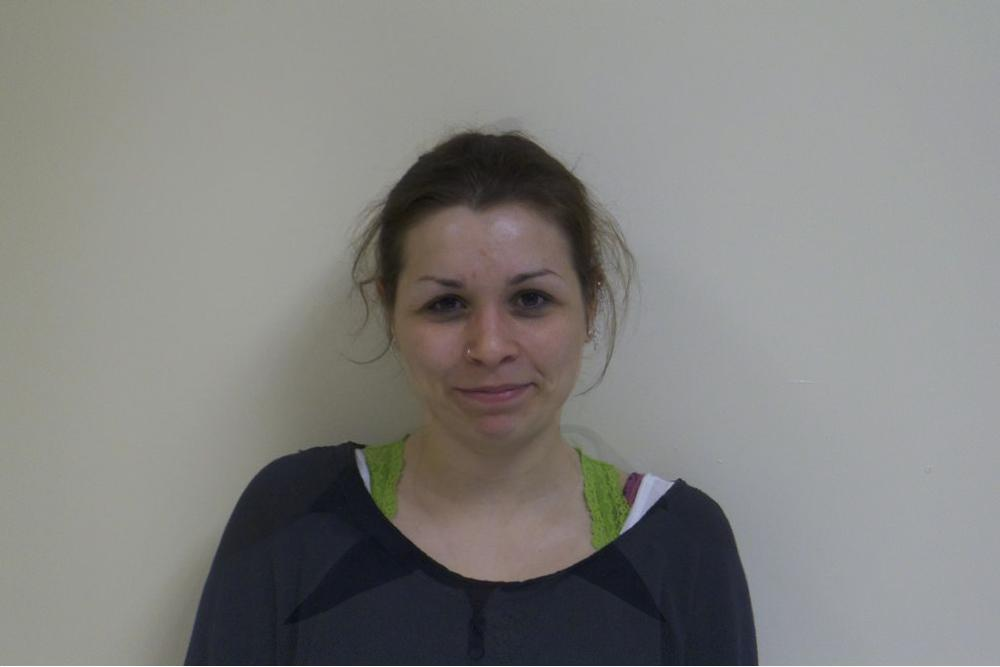
\includegraphics[scale=0.06]{figs/frames/morph_steinkirch_tangatur_07.jpg} 
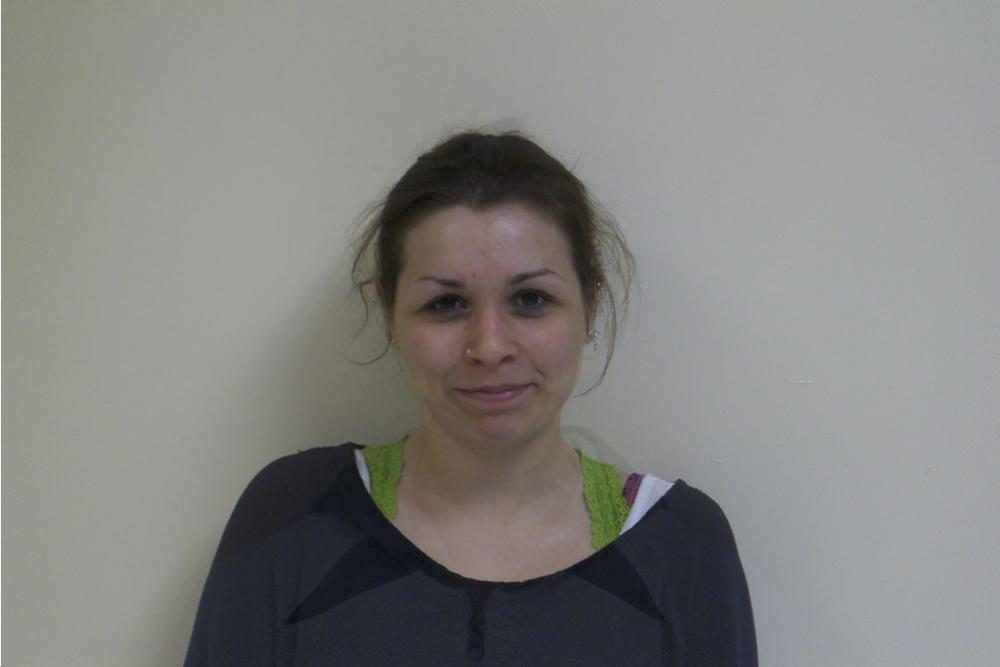
\includegraphics[scale=0.06]{figs/frames/morph_steinkirch_tangatur_08.jpg}  
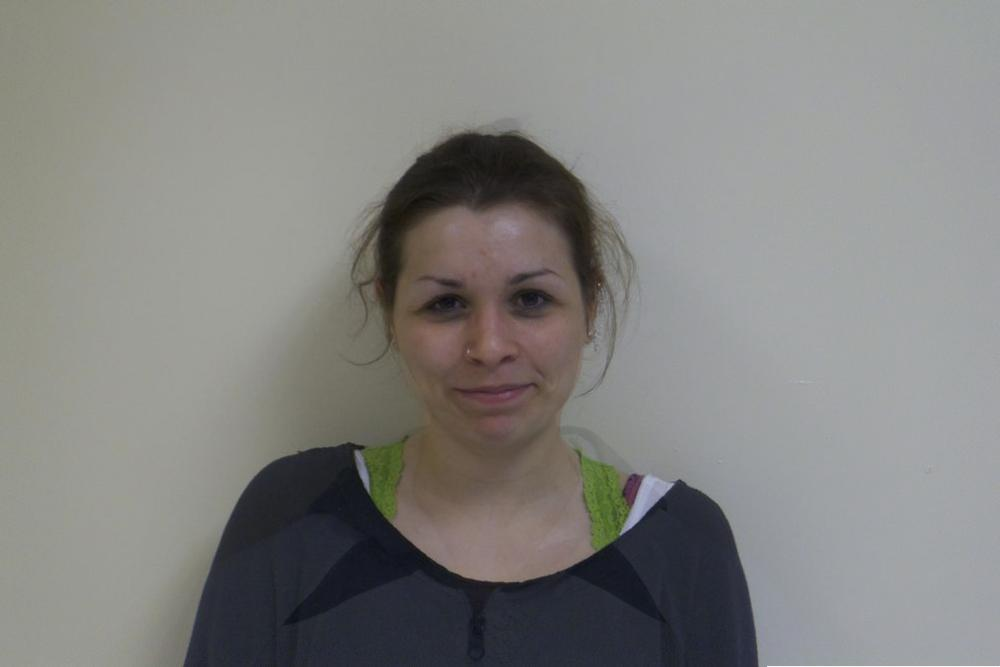
\includegraphics[scale=0.06]{figs/frames/morph_steinkirch_tangatur_09.jpg} 
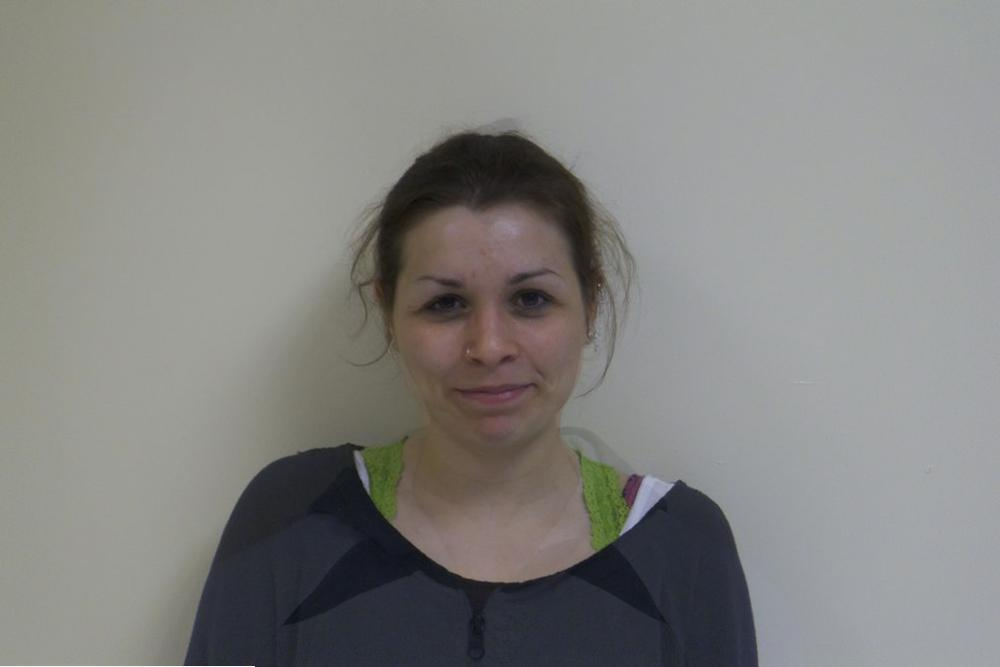
\includegraphics[scale=0.06]{figs/frames/morph_steinkirch_tangatur_10.jpg} 
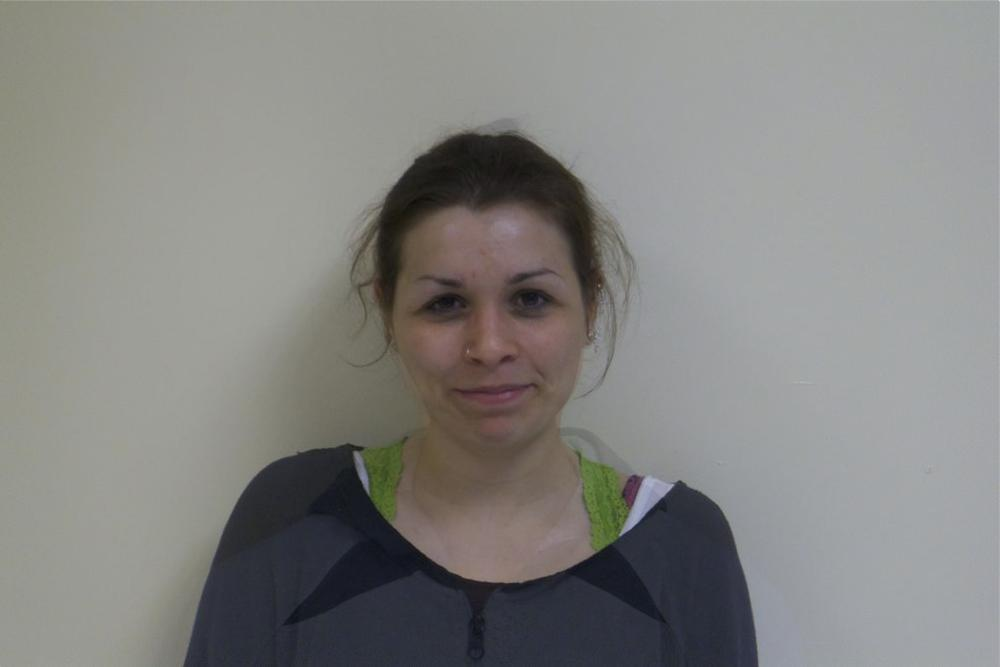
\includegraphics[scale=0.06]{figs/frames/morph_steinkirch_tangatur_11.jpg} 
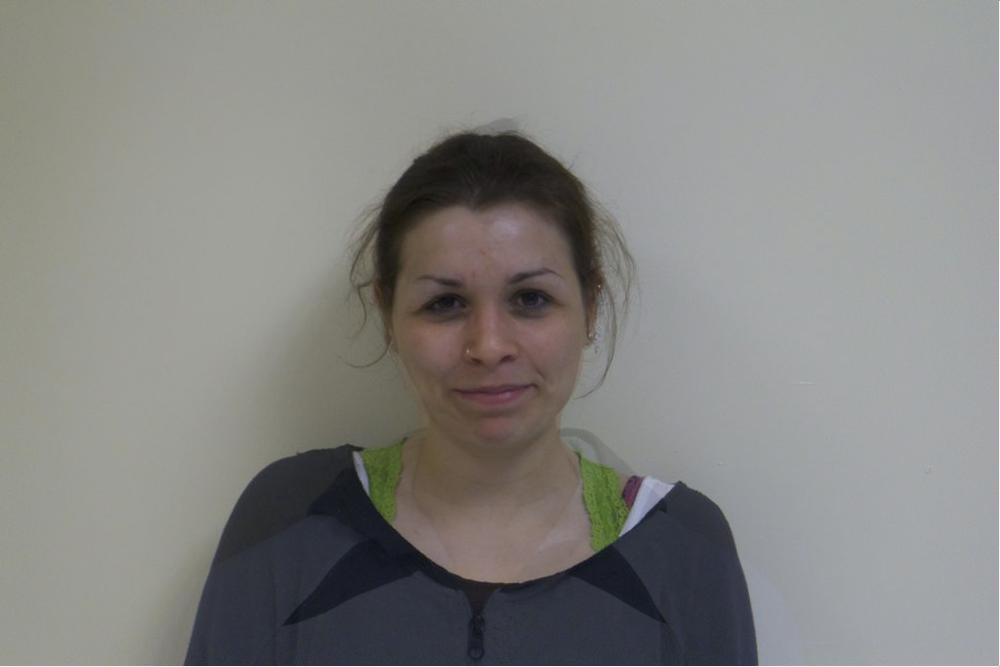
\includegraphics[scale=0.06]{figs/frames/morph_steinkirch_tangatur_12.jpg} 
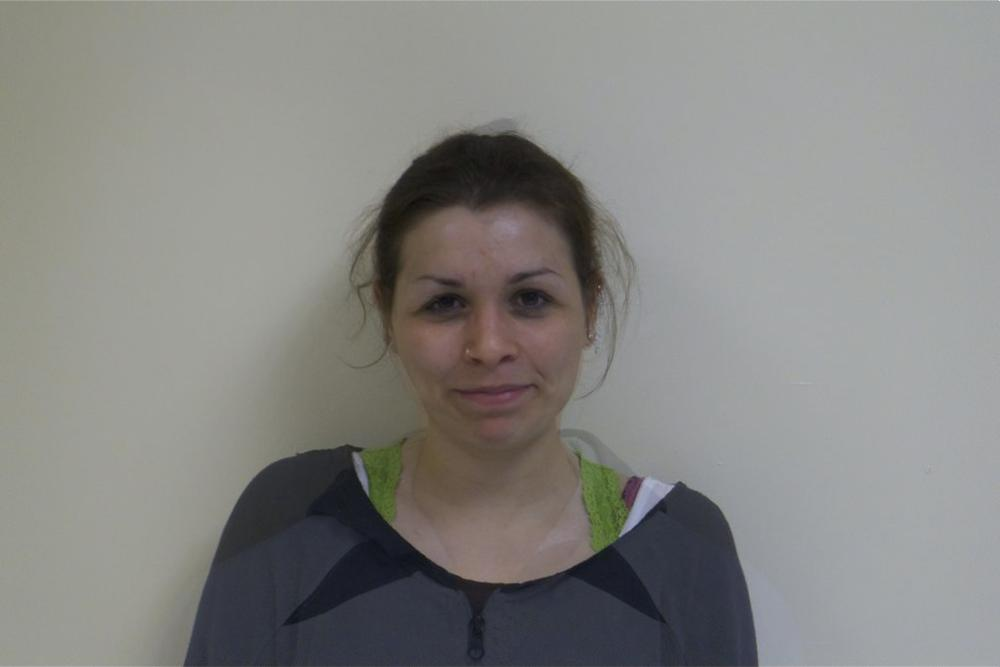
\includegraphics[scale=0.06]{figs/frames/morph_steinkirch_tangatur_13.jpg} 
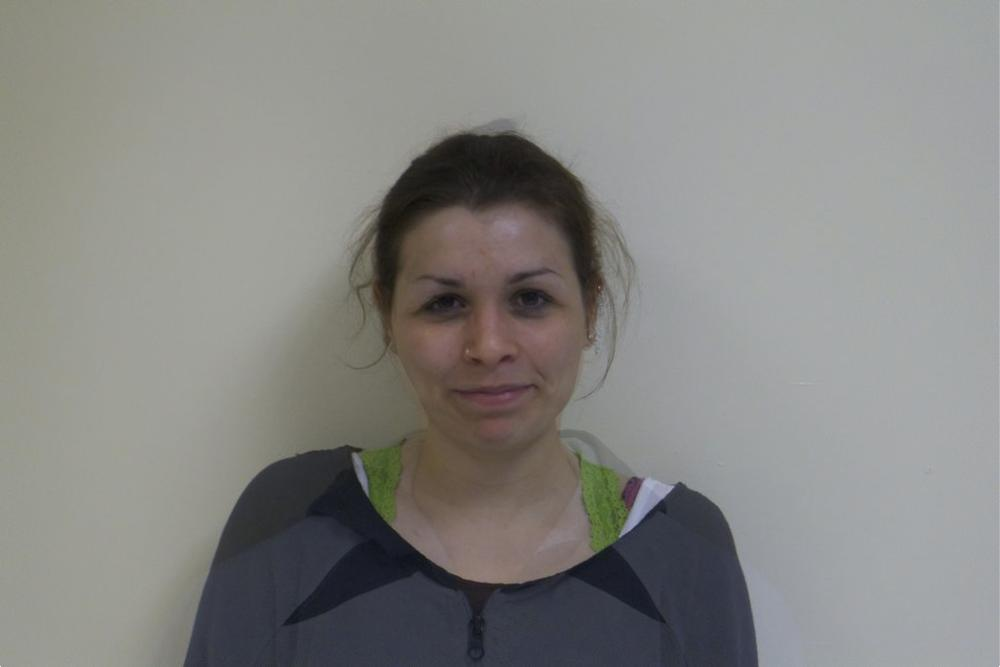
\includegraphics[scale=0.06]{figs/frames/morph_steinkirch_tangatur_14.jpg} 
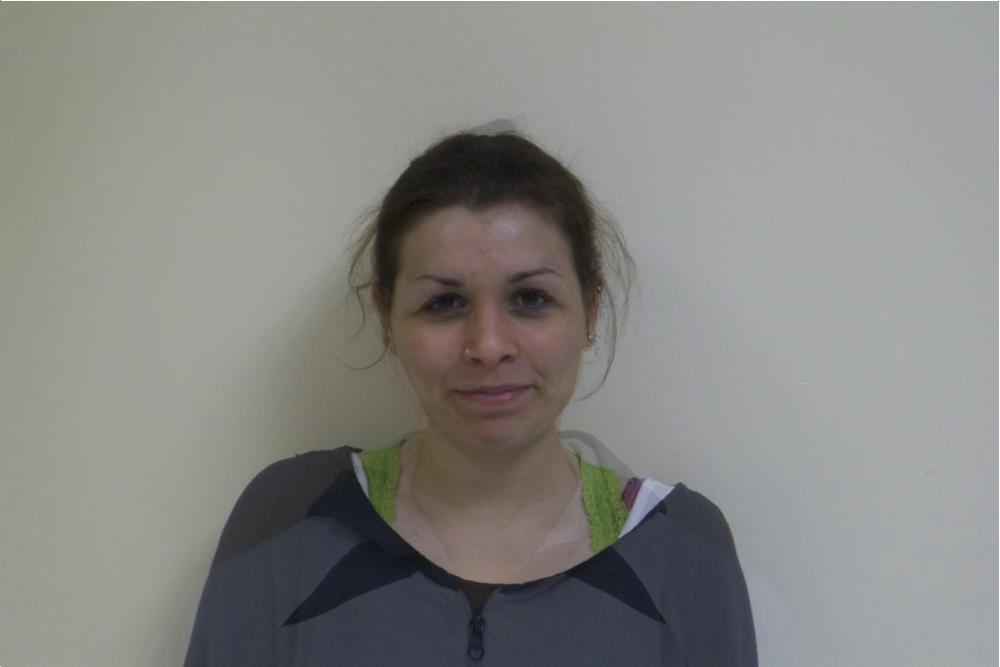
\includegraphics[scale=0.06]{figs/frames/morph_steinkirch_tangatur_15.jpg}  
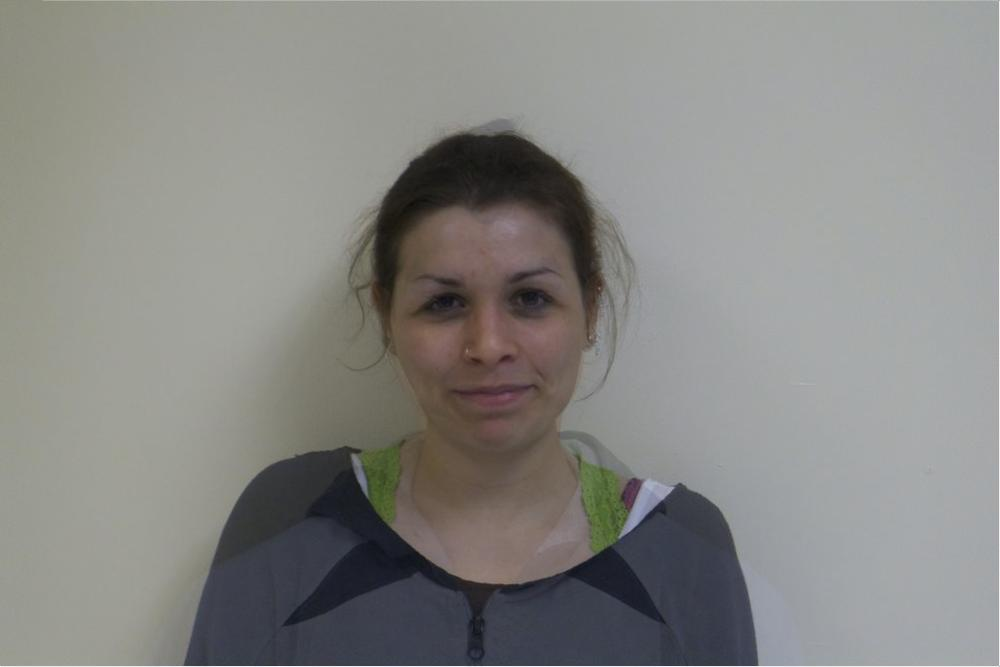
\includegraphics[scale=0.06]{figs/frames/morph_steinkirch_tangatur_16.jpg} 
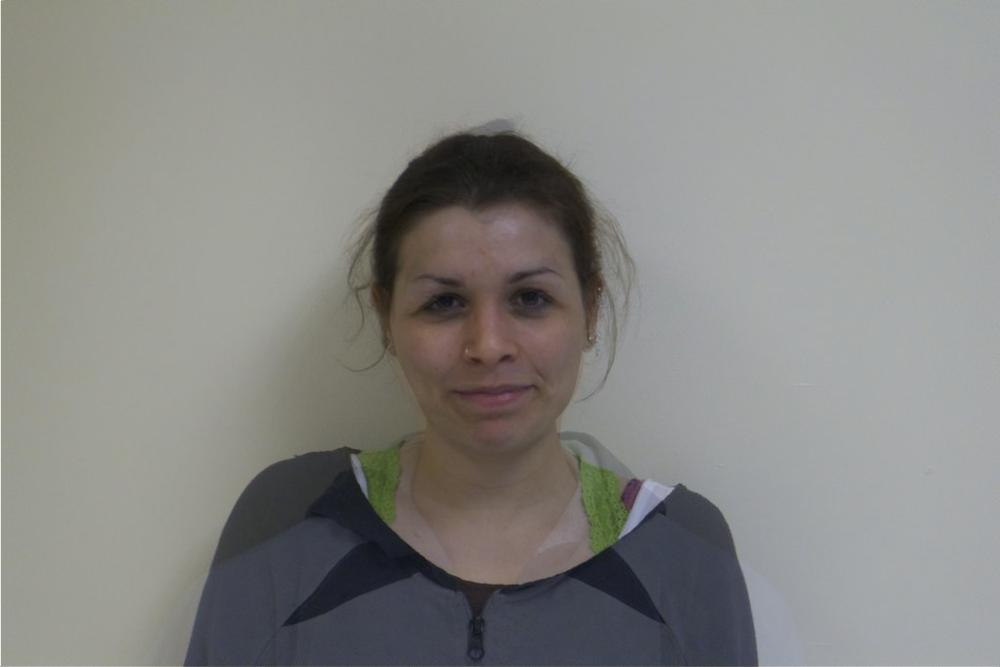
\includegraphics[scale=0.06]{figs/frames/morph_steinkirch_tangatur_17.jpg} 
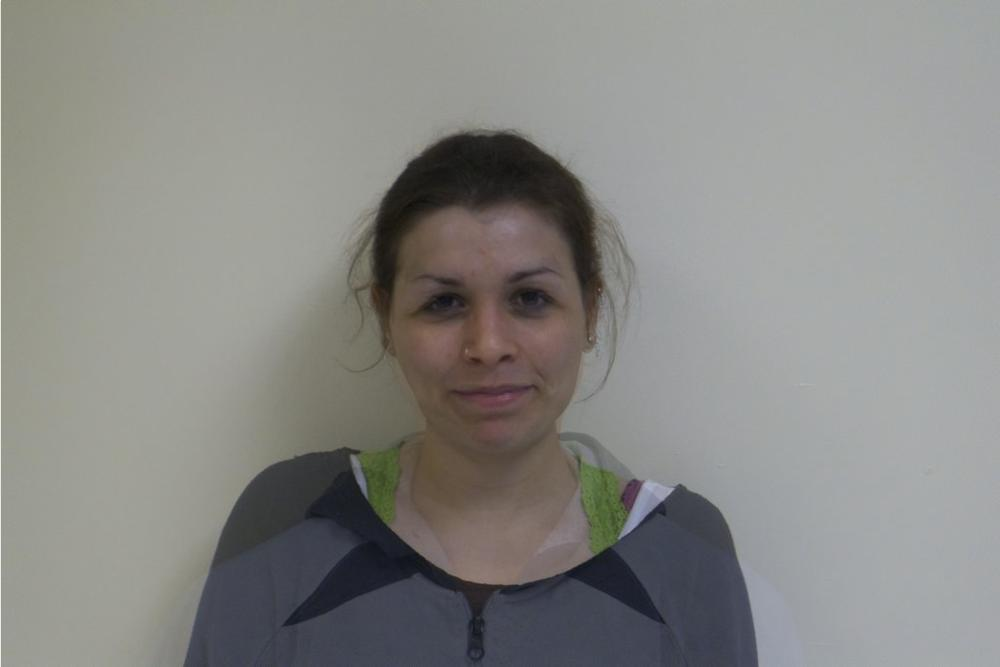
\includegraphics[scale=0.06]{figs/frames/morph_steinkirch_tangatur_18.jpg} 
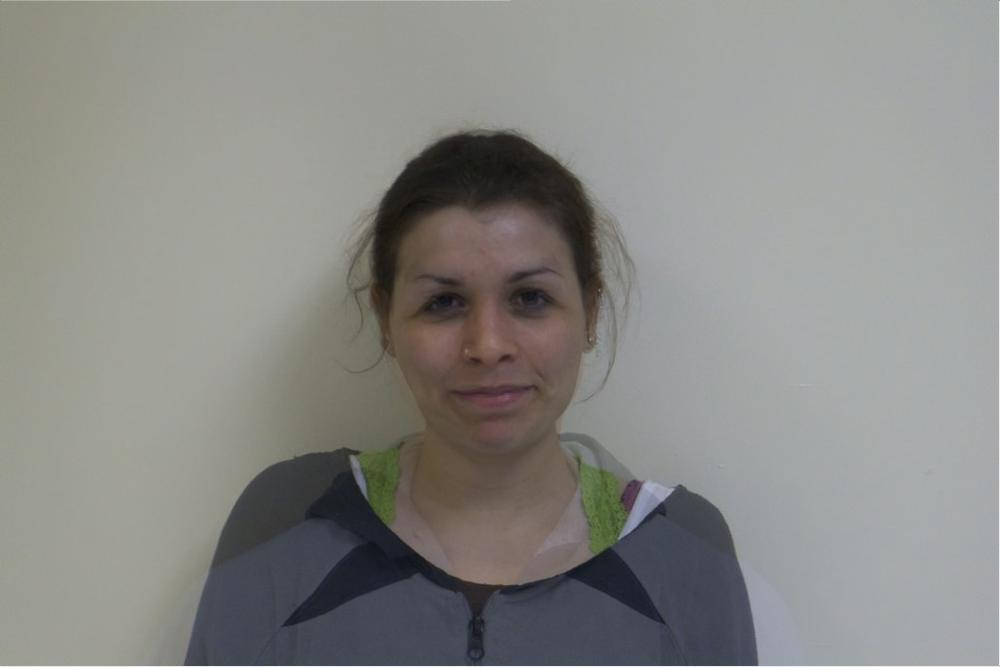
\includegraphics[scale=0.06]{figs/frames/morph_steinkirch_tangatur_19.jpg} 
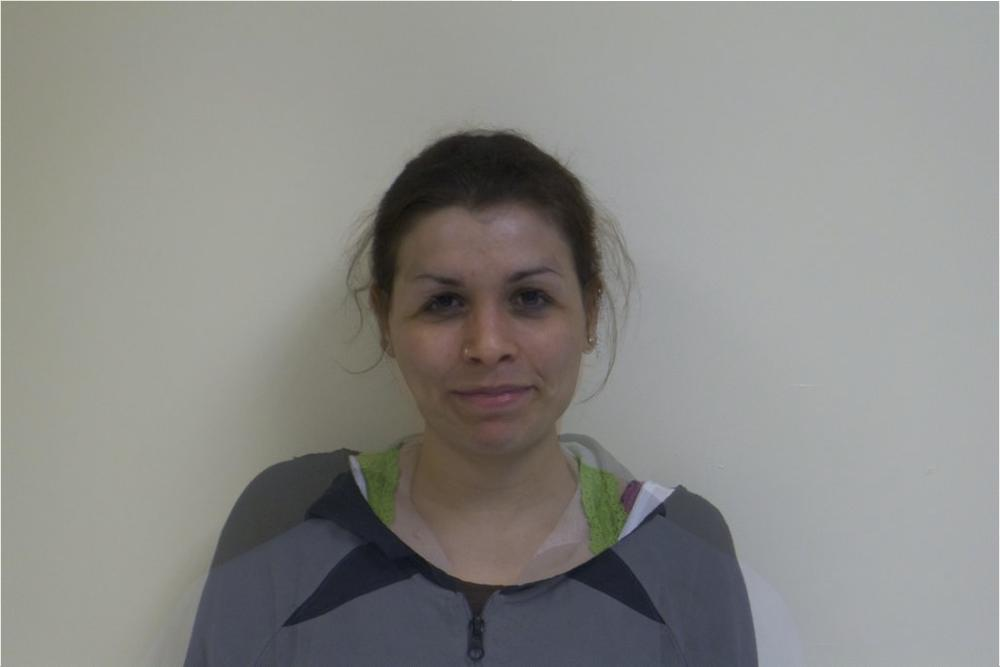
\includegraphics[scale=0.06]{figs/frames/morph_steinkirch_tangatur_20.jpg} 
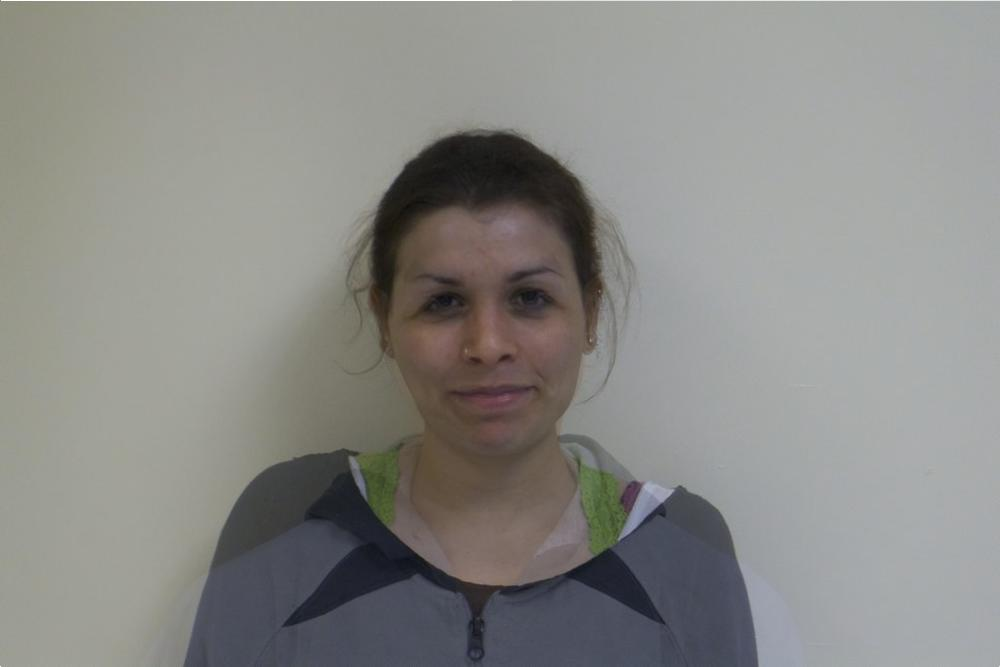
\includegraphics[scale=0.06]{figs/frames/morph_steinkirch_tangatur_21.jpg} 
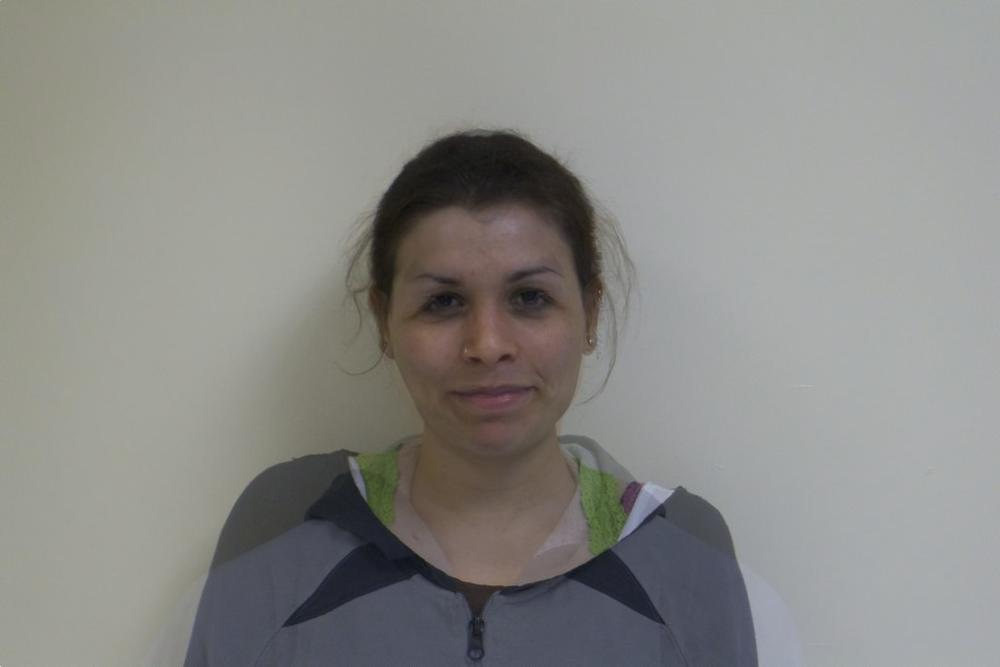
\includegraphics[scale=0.06]{figs/frames/morph_steinkirch_tangatur_22.jpg}  
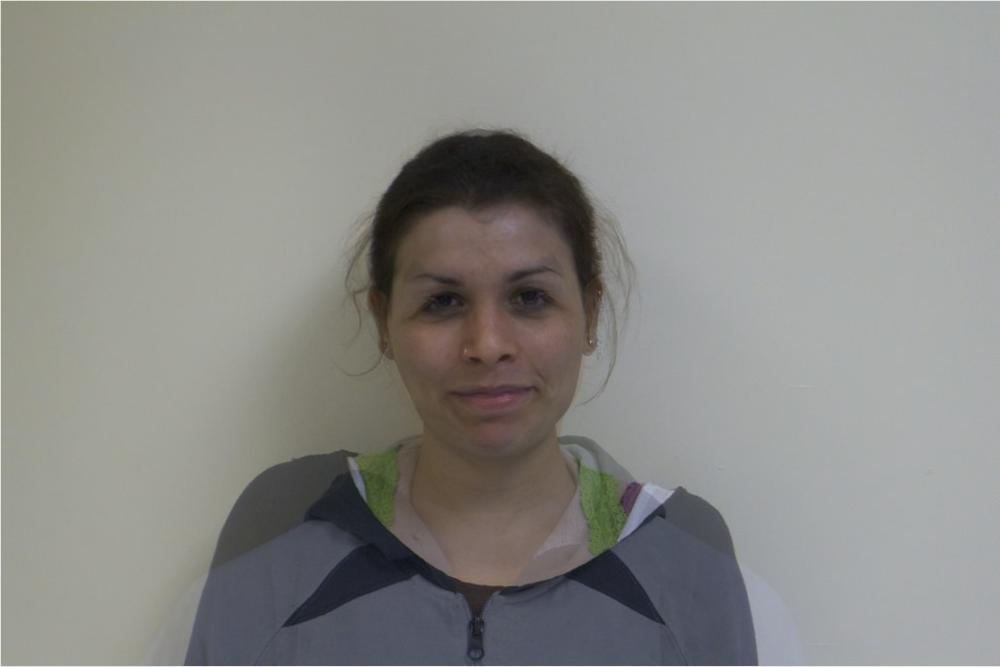
\includegraphics[scale=0.06]{figs/frames/morph_steinkirch_tangatur_23.jpg} 
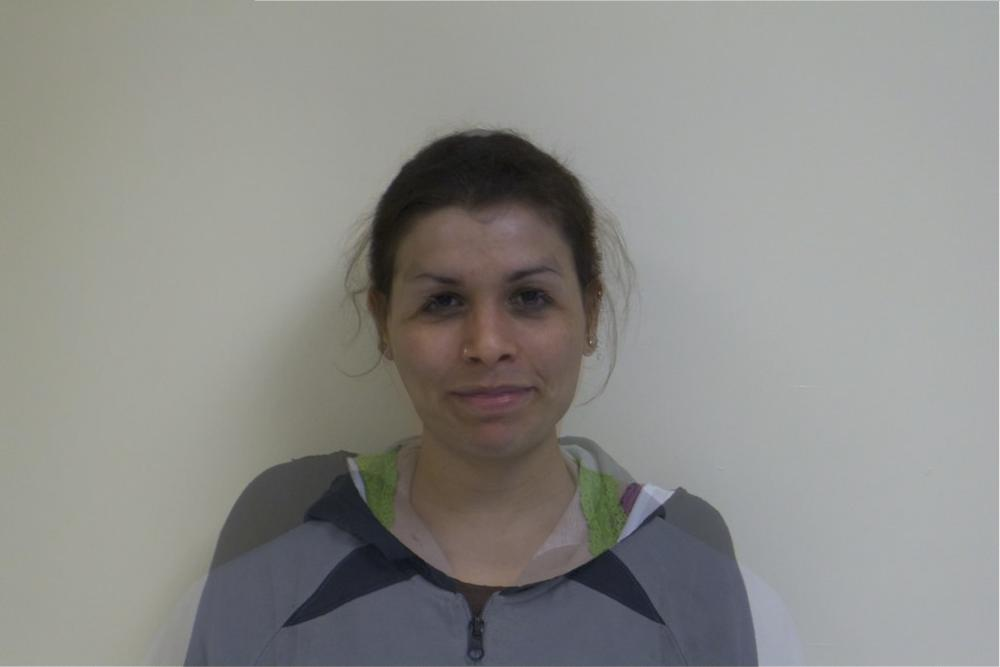
\includegraphics[scale=0.06]{figs/frames/morph_steinkirch_tangatur_24.jpg} 
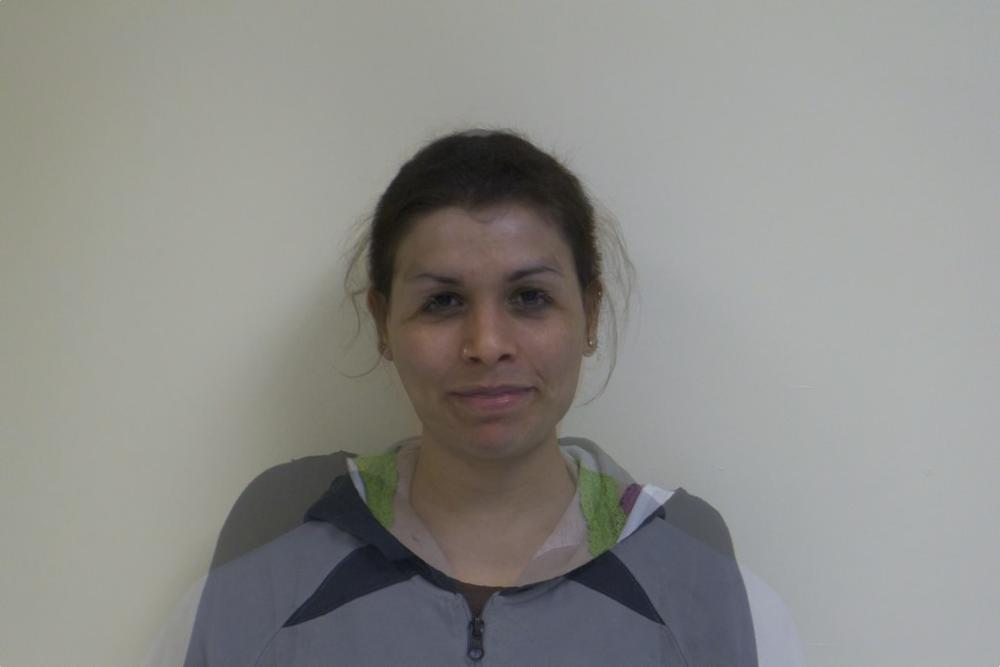
\includegraphics[scale=0.06]{figs/frames/morph_steinkirch_tangatur_25.jpg} 
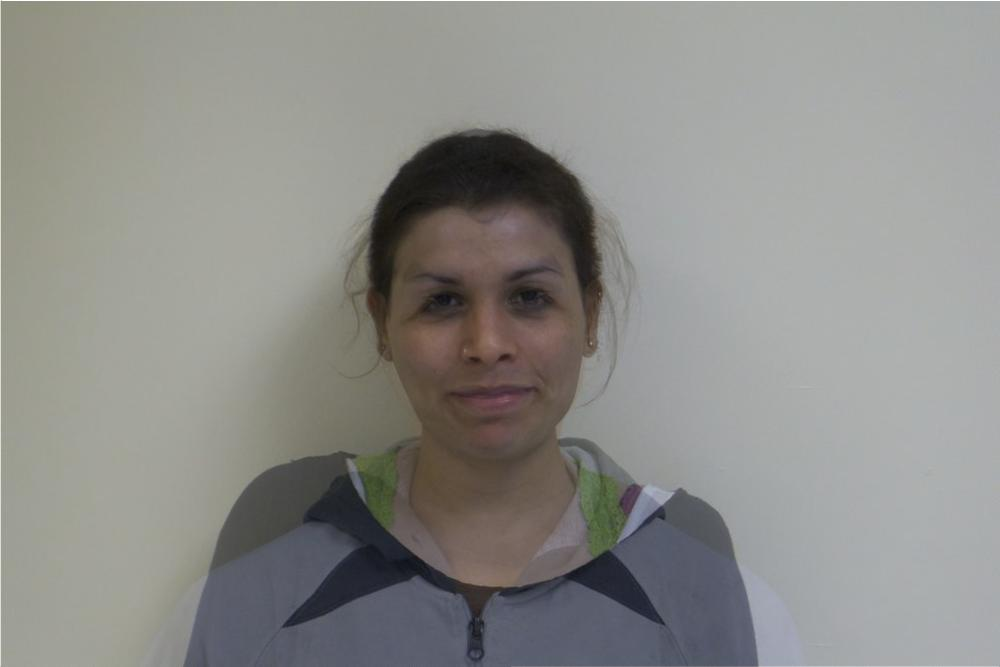
\includegraphics[scale=0.06]{figs/frames/morph_steinkirch_tangatur_26.jpg} 
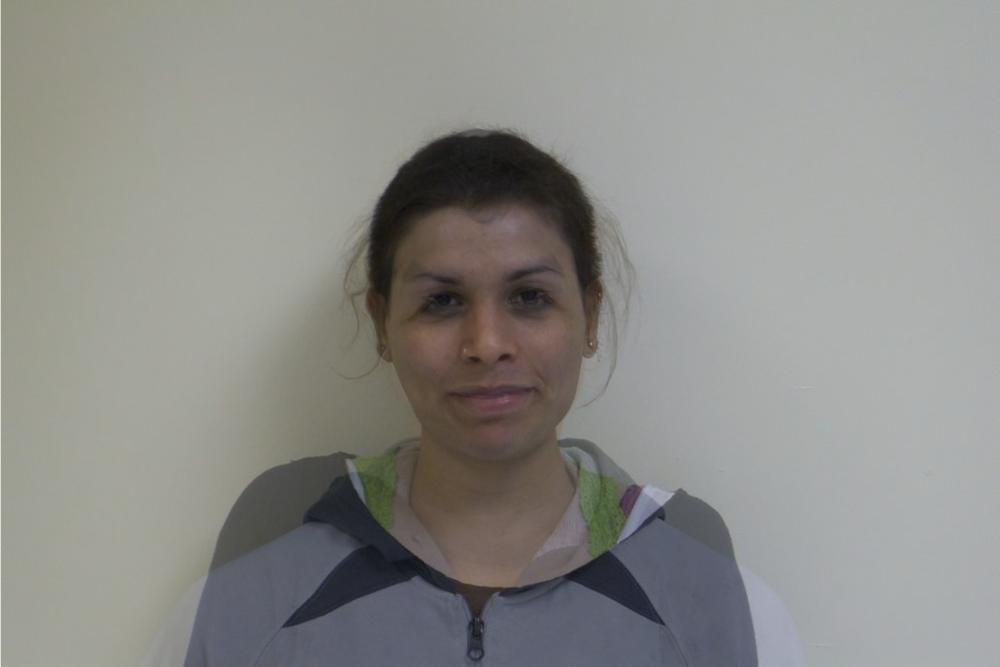
\includegraphics[scale=0.06]{figs/frames/morph_steinkirch_tangatur_27.jpg} 
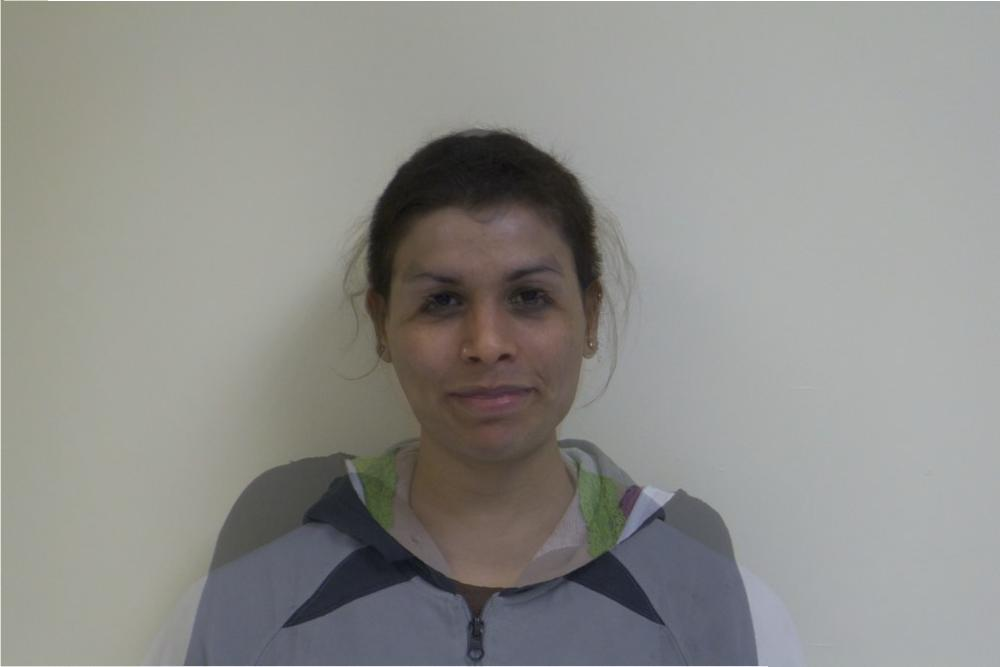
\includegraphics[scale=0.06]{figs/frames/morph_steinkirch_tangatur_28.jpg} 
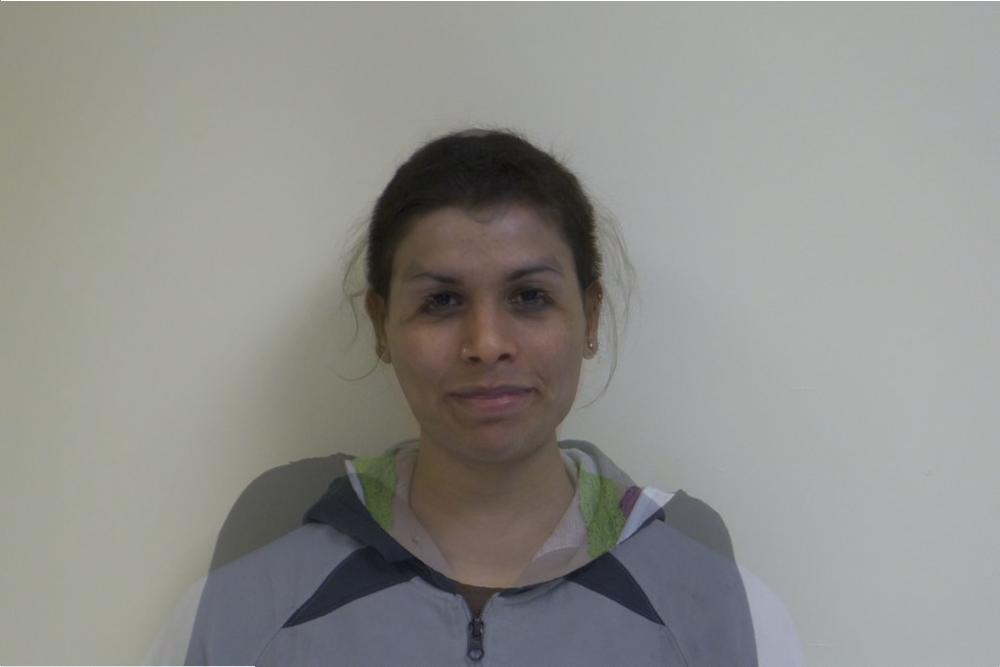
\includegraphics[scale=0.06]{figs/frames/morph_steinkirch_tangatur_29.jpg}  
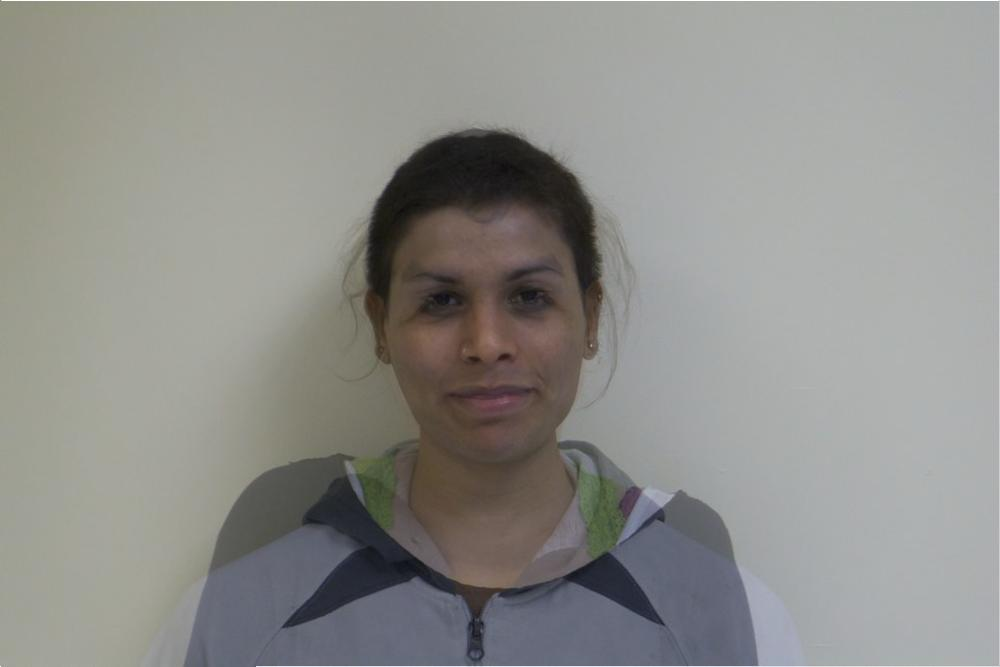
\includegraphics[scale=0.06]{figs/frames/morph_steinkirch_tangatur_30.jpg} 
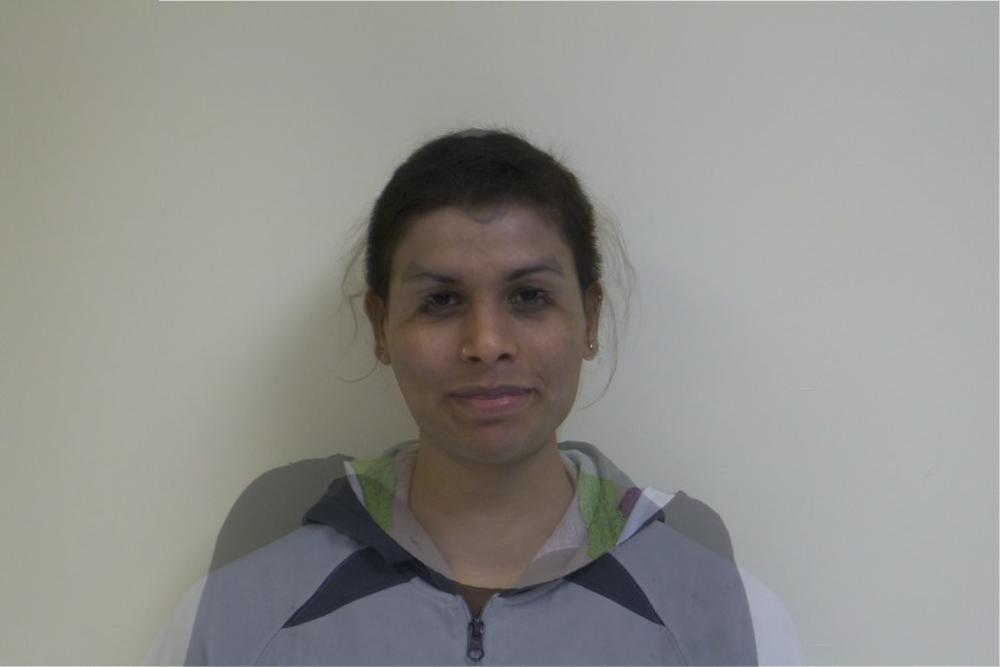
\includegraphics[scale=0.06]{figs/frames/morph_steinkirch_tangatur_31.jpg} 
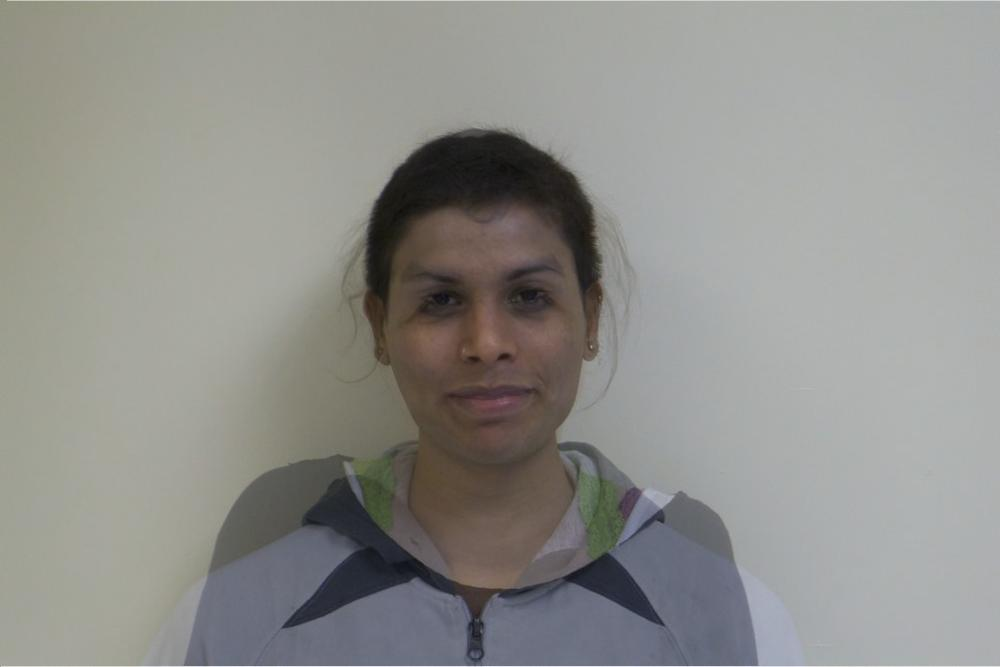
\includegraphics[scale=0.06]{figs/frames/morph_steinkirch_tangatur_32.jpg} 
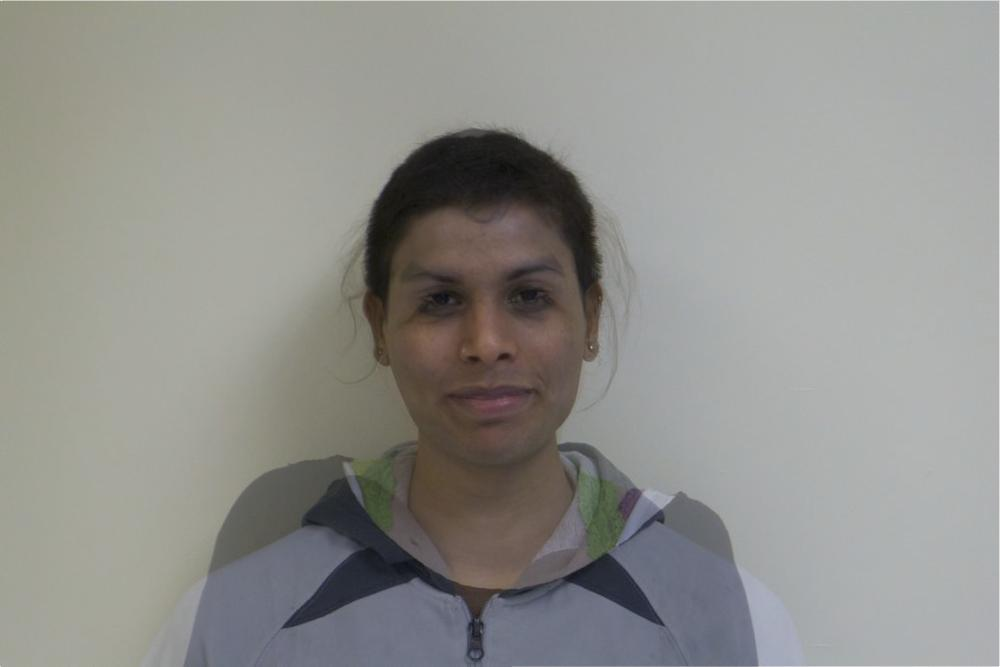
\includegraphics[scale=0.06]{figs/frames/morph_steinkirch_tangatur_33.jpg} 
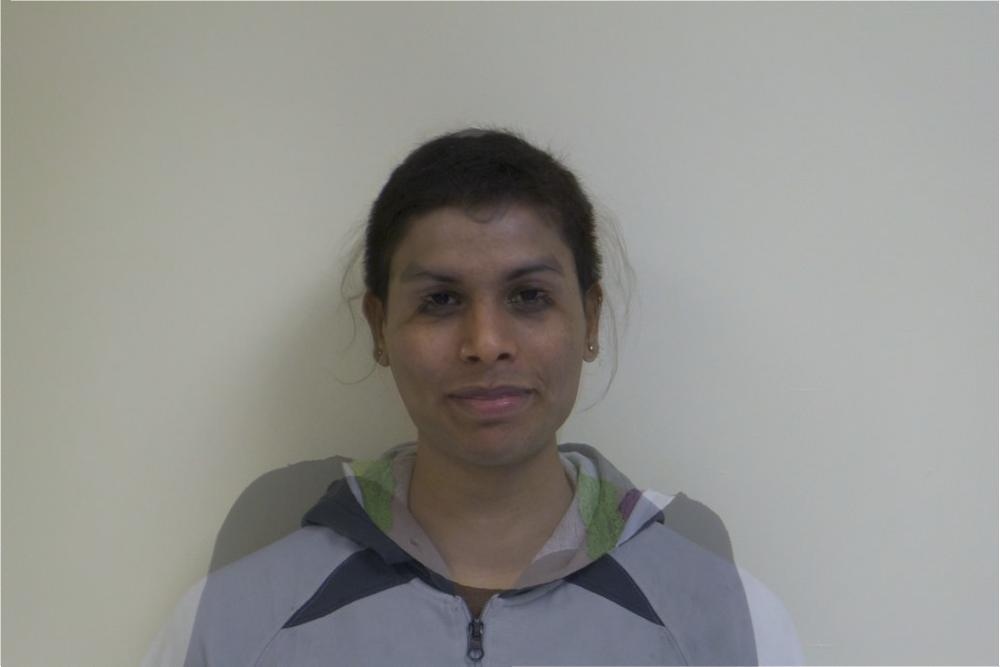
\includegraphics[scale=0.06]{figs/frames/morph_steinkirch_tangatur_34.jpg} 
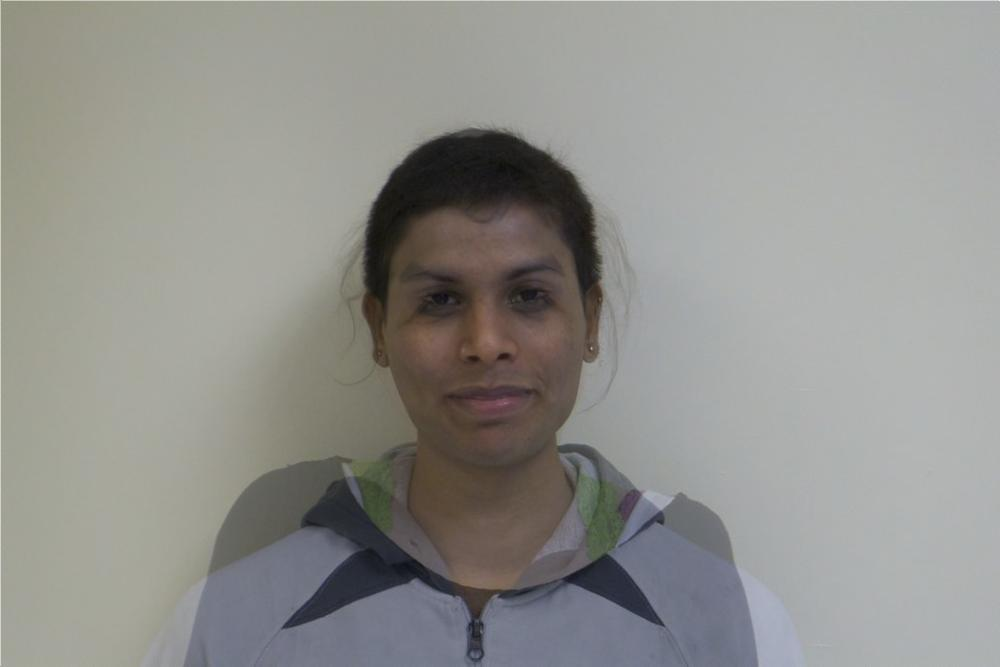
\includegraphics[scale=0.06]{figs/frames/morph_steinkirch_tangatur_35.jpg} 
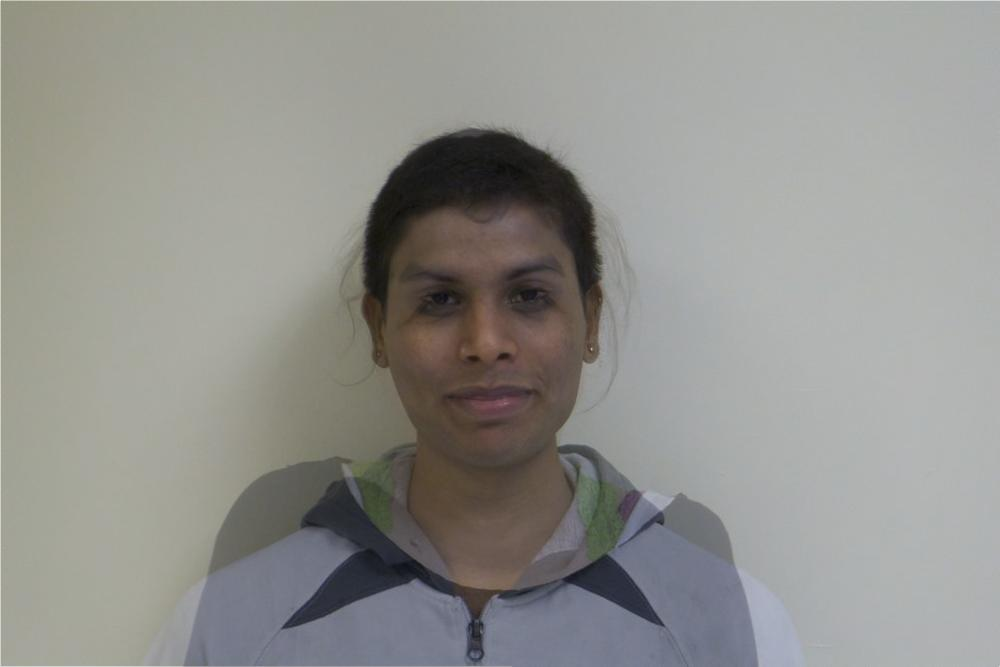
\includegraphics[scale=0.06]{figs/frames/morph_steinkirch_tangatur_36.jpg}  
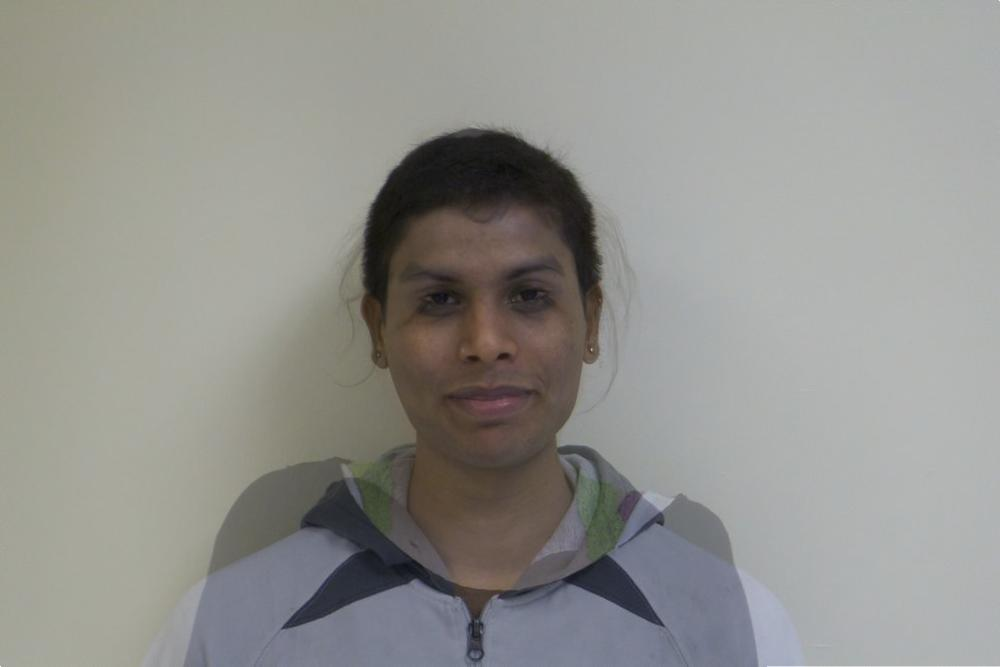
\includegraphics[scale=0.06]{figs/frames/morph_steinkirch_tangatur_37.jpg} 
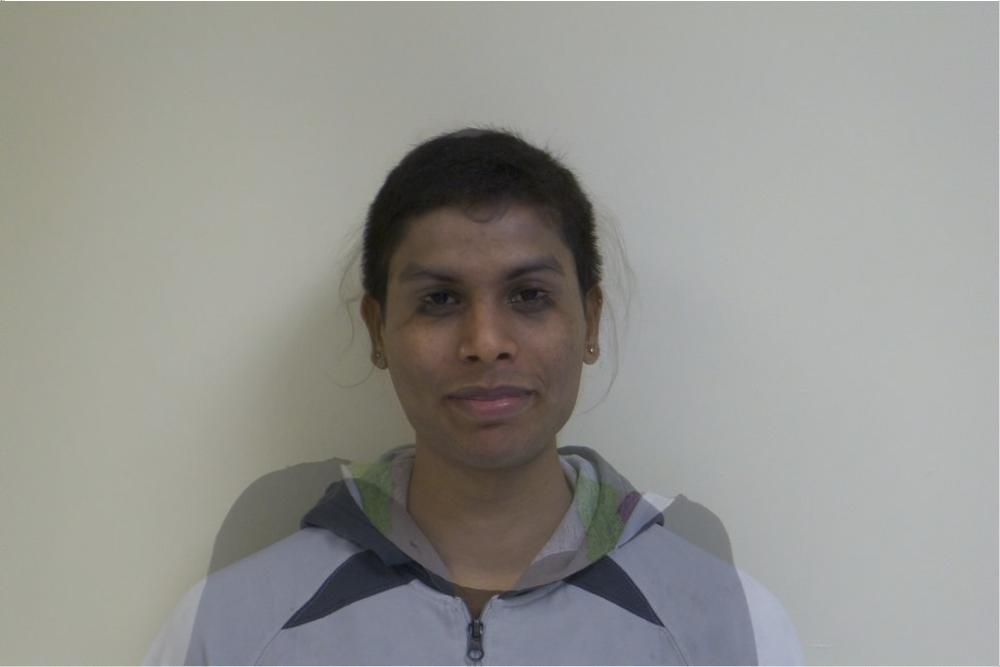
\includegraphics[scale=0.06]{figs/frames/morph_steinkirch_tangatur_38.jpg} 
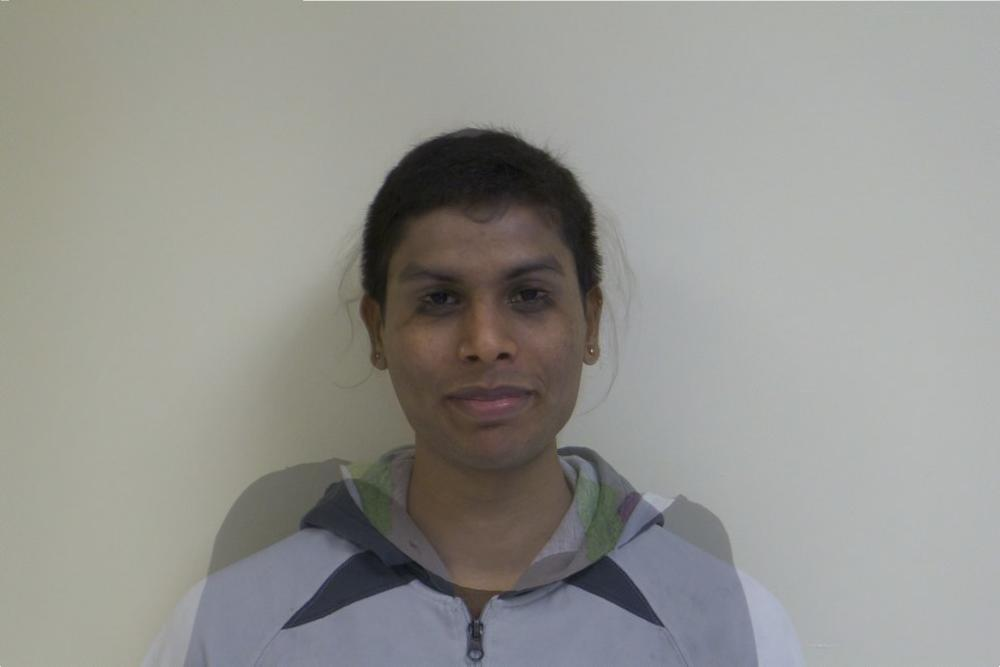
\includegraphics[scale=0.06]{figs/frames/morph_steinkirch_tangatur_39.jpg} 
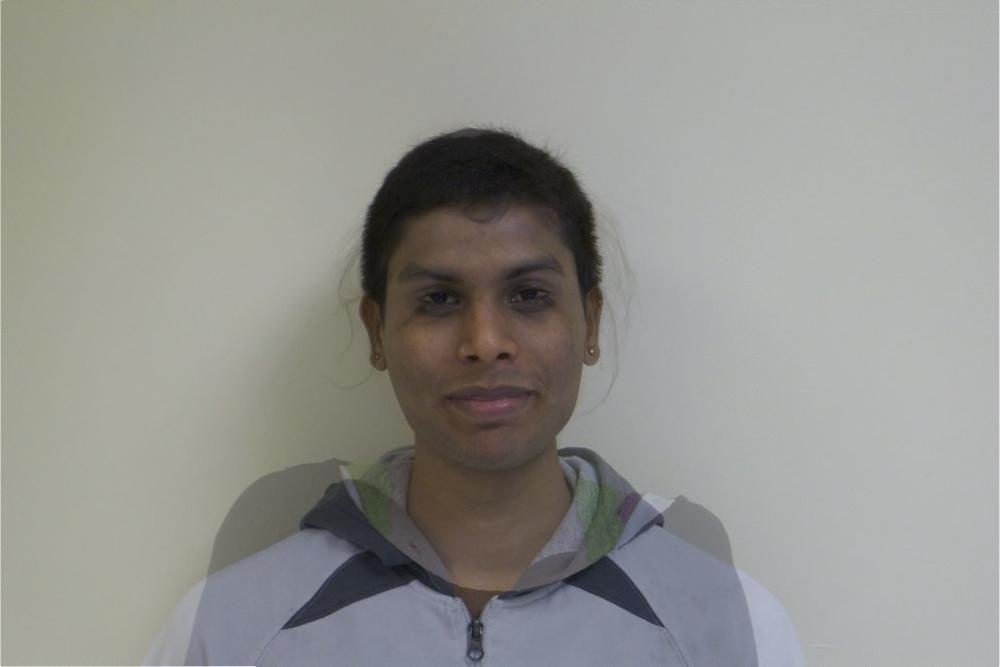
\includegraphics[scale=0.06]{figs/frames/morph_steinkirch_tangatur_40.jpg} 
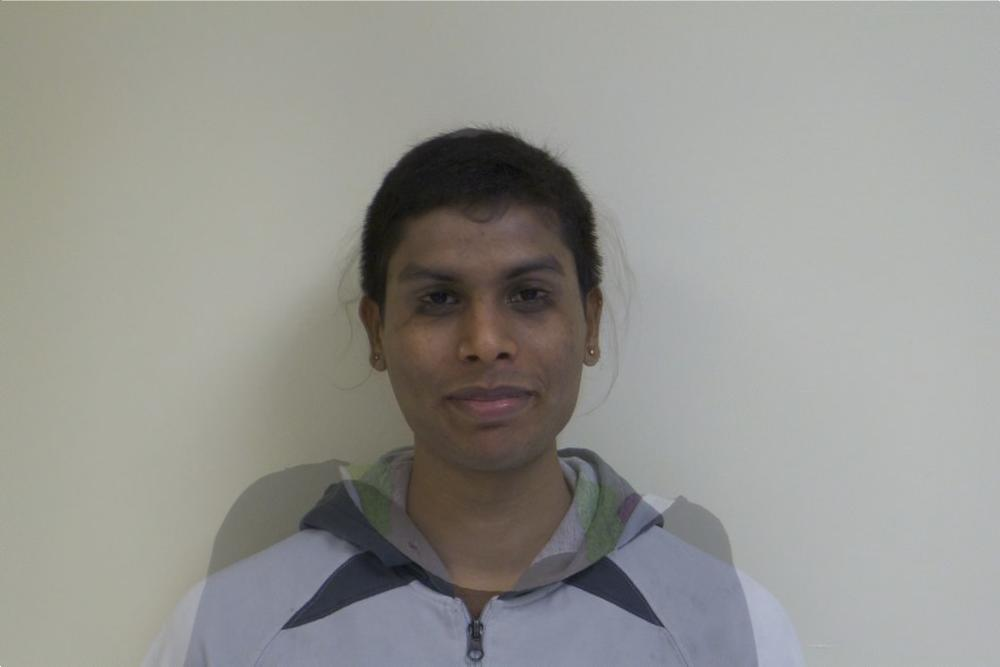
\includegraphics[scale=0.06]{figs/frames/morph_steinkirch_tangatur_41.jpg} 
\includegraphics[scale=0.06]{figs/frames/morph_steinkirch_tangatur_42.jpg} 
\includegraphics[scale=0.06]{figs/frames/morph_steinkirch_tangatur_43.jpg}  
\includegraphics[scale=0.06]{figs/frames/morph_steinkirch_tangatur_44.jpg} 
\includegraphics[scale=0.06]{figs/frames/morph_steinkirch_tangatur_45.jpg} 
\includegraphics[scale=0.06]{figs/frames/morph_steinkirch_tangatur_46.jpg} 
\includegraphics[scale=0.06]{figs/frames/morph_steinkirch_tangatur_47.jpg} 
\includegraphics[scale=0.06]{figs/frames/morph_steinkirch_tangatur_48.jpg} 
\includegraphics[scale=0.06]{figs/frames/morph_steinkirch_tangatur_49.jpg} 
\includegraphics[scale=0.06]{figs/frames/morph_steinkirch_tangatur_50.jpg}  
\includegraphics[scale=0.06]{figs/frames/morph_steinkirch_tangatur_51.jpg} 
\includegraphics[scale=0.06]{figs/frames/morph_steinkirch_tangatur_52.jpg} 
\includegraphics[scale=0.06]{figs/frames/morph_steinkirch_tangatur_53.jpg} 
\includegraphics[scale=0.06]{figs/frames/morph_steinkirch_tangatur_54.jpg} 
\includegraphics[scale=0.06]{figs/frames/morph_steinkirch_tangatur_55.jpg} 
\includegraphics[scale=0.06]{figs/frames/morph_steinkirch_tangatur_56.jpg} 
\includegraphics[scale=0.06]{figs/frames/morph_steinkirch_tangatur_57.jpg}  
\includegraphics[scale=0.06]{figs/frames/morph_steinkirch_tangatur_58.jpg} 
\includegraphics[scale=0.06]{figs/frames/morph_steinkirch_tangatur_59.jpg} 
\includegraphics[scale=0.06]{figs/frames/morph_steinkirch_tangatur_60.jpg} 
\includegraphics[scale=0.06]{figs/frames/morph_steinkirch_tangatur_61.jpg} 


\caption{Face morphism: the initial and final images to be morphed and the 58 intermediate frames generate to morph them.}
\label{frames}
\end{center}
\end{figure}



\newpage

	
\section{Calculating the Mean Face}

Utilizing the previous techniques we calculate the mean face for the whole class. The result can be seen in the Fig. \ref{mean}.

\quad

\begin{figure}[H]
\begin{center}
\includegraphics[scale=0.4]{figs/mean.jpg}  
\caption{Example of the mean face for many face images (class pictures).}
\label{mean}
\end{center}
\end{figure}


\newpage



\section{Fun Example: Caricatures of a Face Image}

The face morphism techniques can be use to produce fun results. As a first example, we utilize each of the face points mapping from the entire class to create caricatures for a unique face image. The results can be seen in the Fig. \ref{mean-me}.

\quad


Since the map of the other faces is not made as an exact caricature mapping but rather it is just a coincident characterization, some pictures exhibits artifacts (and some does not). The example here showed how to use many different mapping labels to the same picture, however to be able to reproduce specifics caricature features without producing any artifacts, the correct way would be to write a new mapping with coordinates modifications to only  the specific facial parts we want to exaggerate, \eg the nose or the eyes, etc. However this examples illustrate the point well. 

\begin{figure}[H]
\begin{center}
\includegraphics[scale=0.17]{figs/caricatures/fun_02.jpg}  
\includegraphics[scale=0.17]{figs/caricatures/fun_03.jpg}  
\includegraphics[scale=0.17]{figs/caricatures/fun_04.jpg}  
\includegraphics[scale=0.17]{figs/caricatures/fun_15.jpg} 


 \end{center}
\end{figure}
\begin{figure}[H]
\begin{center}
\includegraphics[scale=0.17]{figs/caricatures/fun_05.jpg}  
\includegraphics[scale=0.17]{figs/caricatures/fun_06.jpg}  
\includegraphics[scale=0.17]{figs/caricatures/fun_07.jpg}  
\includegraphics[scale=0.17]{figs/caricatures/fun_08.jpg}  
\includegraphics[scale=0.17]{figs/caricatures/fun_09.jpg}  
\includegraphics[scale=0.17]{figs/caricatures/fun_10.jpg} 
\includegraphics[scale=0.17]{figs/caricatures/fun_11.jpg}  
\includegraphics[scale=0.17]{figs/caricatures/fun_12.jpg}  
\includegraphics[scale=0.17]{figs/caricatures/fun_13.jpg}  
\includegraphics[scale=0.17]{figs/caricatures/fun_14.jpg}
    
\caption{Caricatures as examples of the face morphism techniques.}
\label{mean-me}
\end{center}
\end{figure}

\newpage

\section{Fun Example: Zombie Boyfriend}

Utilizing the above techniques for face morphism, we created a smooth transformation of a human face image to an image of  a monster (zombie). We see some small artifacts due the warping of the background and a way to overcome this problem is apply a final blender transformation. The intermediate results are shown in the Fig. \ref{zombie} and a final video of the result can be seen at \cite{video-zombie}.

\quad

\begin{figure}[H]
\begin{center}
\includegraphics[scale=0.08]{figs/zombie/zombie_bf_01.jpg} 
\includegraphics[scale=0.08]{figs/zombie/zombie_bf_02.jpg} 
\includegraphics[scale=0.08]{figs/zombie/zombie_bf_03.jpg} 
\includegraphics[scale=0.08]{figs/zombie/zombie_bf_04.jpg} 
\includegraphics[scale=0.08]{figs/zombie/zombie_bf_05.jpg} 
\includegraphics[scale=0.08]{figs/zombie/zombie_bf_06.jpg} 
\includegraphics[scale=0.08]{figs/zombie/zombie_bf_07.jpg} 
\includegraphics[scale=0.08]{figs/zombie/zombie_bf_08.jpg} 
\includegraphics[scale=0.08]{figs/zombie/zombie_bf_09.jpg} 
\includegraphics[scale=0.08]{figs/zombie/zombie_bf_10.jpg} 
\includegraphics[scale=0.08]{figs/zombie/zombie_bf_11.jpg}
\includegraphics[scale=0.08]{figs/zombie/zombie_bf_12.jpg} 
\includegraphics[scale=0.08]{figs/zombie/zombie_bf_13.jpg} 
\includegraphics[scale=0.08]{figs/zombie/zombie_bf_14.jpg} 
\includegraphics[scale=0.08]{figs/zombie/zombie_bf_15.jpg} 
\includegraphics[scale=0.08]{figs/zombie/zombie_bf_16.jpg} 
\includegraphics[scale=0.08]{figs/zombie/zombie_bf_17.jpg} 
\includegraphics[scale=0.08]{figs/zombie/zombie_bf_18.jpg} 
\includegraphics[scale=0.08]{figs/zombie/zombie_bf_19.jpg} 
\includegraphics[scale=0.08]{figs/zombie/zombie_bf_20.jpg} 
\caption{Face transformation to a monster as an example of the face morphism techniques.}
\label{zombie}
\end{center}
\end{figure}





\newpage


%%%%%%%%%%%%%%%%%%%%%%%%%%%%%%%%%%%%%%%%%%%%%%%%%%%%%%%%%%%%%%%%%%%%%%%%%%%%%%%%%%%%%%%%%%%%%%
%%%%%%%%%%%%%%%%%%%%%%%%%%%%%%%%%%%%%		Ref		%%%%%%%%%%%%%%%%%%%%%%%%%%%%%%%%%%%%%%%%%%
%%%%%%%%%%%%%%%%%%%%%%%%%%%%%%%%%%%%%%%%%%%%%%%%%%%%%%%%%%%%%%%%%%%%%%%%%%%%%%%%%%%%%%%%%%%%%%



\begin{thebibliography}{}

\bibitem{tamara}{\it Tamara Berg's Class}, {\it http://www.tamaraberg.com/teaching/Spring13/compphotog/3}

\bibitem{video-face} {\it Link to a video with the Face Morphism result}, {\texttt http://www.youtube.com/watch?v=sMtAMN6JLho}, 2013

\bibitem{video-zombie} {\it Link to a video with the Face Morphism example (zombie boyfriend)}, {\texttt http://www.youtube.com/watch?v=O5nBHLGvPs}, 2013

\end{thebibliography}



\end{document}

